\documentclass[ xcolor = pdftex, dvipsnames, table ]{beamer}

\usetheme{Berlin}
\usecolortheme{whale}
\setlength{\parskip}{0.1in}
\usepackage{bm}
\usepackage{tikz}
\usepackage{graphicx}
\usepackage{verbatim}
\usepackage{hyperref}
\usepackage{changepage}

%\usepackage{rNames}

%\title{Baysian Nonparametric Estimation of ODEs as Applied to the Stock Recruitment Relationship}
\title{Bias Estimation of Biological Reference Points Under Two-Parameter SRRs}
\author{
Nick Grunloh\\$~$\\
In collaboration with:\\
Dr. E.J. Dick\\
Dr. H. K.H. Lee
}
\date{17 Aug 2022}

\DeclareMathOperator*{\argmin}{\arg\!\min}
\DeclareMathOperator*{\argmax}{\arg\!\max}

%\newenvironment{changemargin}[2]{%
%\begin{list}{}{%
%\setlength{\topsep}{0pt}%
%\setlength{\leftmargin}{#1}%
%\setlength{\rightmargin}{#2}%
%\setlength{\listparindent}{\parindent}%
%\setlength{\itemindent}{\parindent}%
%\setlength{\parsep}{\parskip}%
%}%
%\item[]}{\end{list}}

\begin{document}
%
\begin{frame}
\titlepage
\vspace*{-3cm}
\begin{minipage}[h!]{0.49\textwidth}
\hspace*{-0.25cm}

\includegraphics[width=0.6\textwidth]{noaaText.png}
\end{minipage}
\begin{minipage}[h!]{0.49\textwidth}
\hspace*{2cm}

\includegraphics[width=0.55\textwidth]{slug.jpg}
\end{minipage}
\end{frame}

%
\section{Introduction}
\subsection{}


%
\begin{frame}{General Modeling Structures}
\hspace*{-0.5cm}
\begin{minipage}[h!]{0.49\textwidth}
\begin{align*}
I_t &= q B_t e^\epsilon ~~~ \epsilon\sim N(0, \sigma^2) \\
~\\
\frac{dB(t)}{dt} &= P(B(t);\bm{\theta}) - Z(t)B(t)\\
~\\~\\
RP &: MSY, ~\frac{F_{MSY}}{M}, ~\frac{B_{MSY}}{B_0} 
\end{align*}
\end{minipage}
\begin{minipage}[h!]{0.49\textwidth}
$~$\\\hspace*{0.2cm}
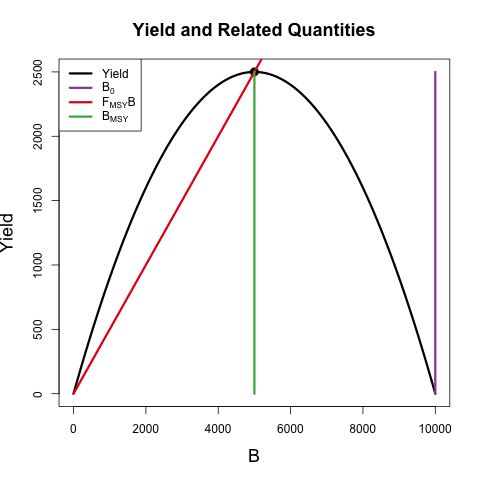
\includegraphics[width=1.2\textwidth]{../advance/plots/yieldRPplus.png}
\end{minipage}
\end{frame}

%
\begin{frame}
\only<1>{
\hspace*{-0.5cm}
\begin{minipage}[h!]{0.59\textwidth}
Conceptually:
\begin{align*}
\frac{F_{MSY}}{M}\in\mathbb{R}^+ ~~~ \frac{B_{MSY}}{B_{0}}\in\left(0, 1\right)
\end{align*}
$~$\\
Mangel et al. 2013, CJFAS:
\begin{itemize}
        \item BH Model: $~ \frac{F_{MSY}}{M}\in\mathbb{R}^+ ~~~ \frac{B_{MSY}}{\bar B(0)}=\frac{1}{F_{MSY}/M+2}$
        \item Similar Constraints for other Two-Parameter Curves %Logistic, Ricker and 
	 % Three-Parameter Relationships Allow Independent RP Estimation
\end{itemize}
$~$\\\vspace{0.075cm}
\end{minipage}
\begin{minipage}[h!]{0.39\textwidth}
$~$\\
\hspace*{-0.3cm}
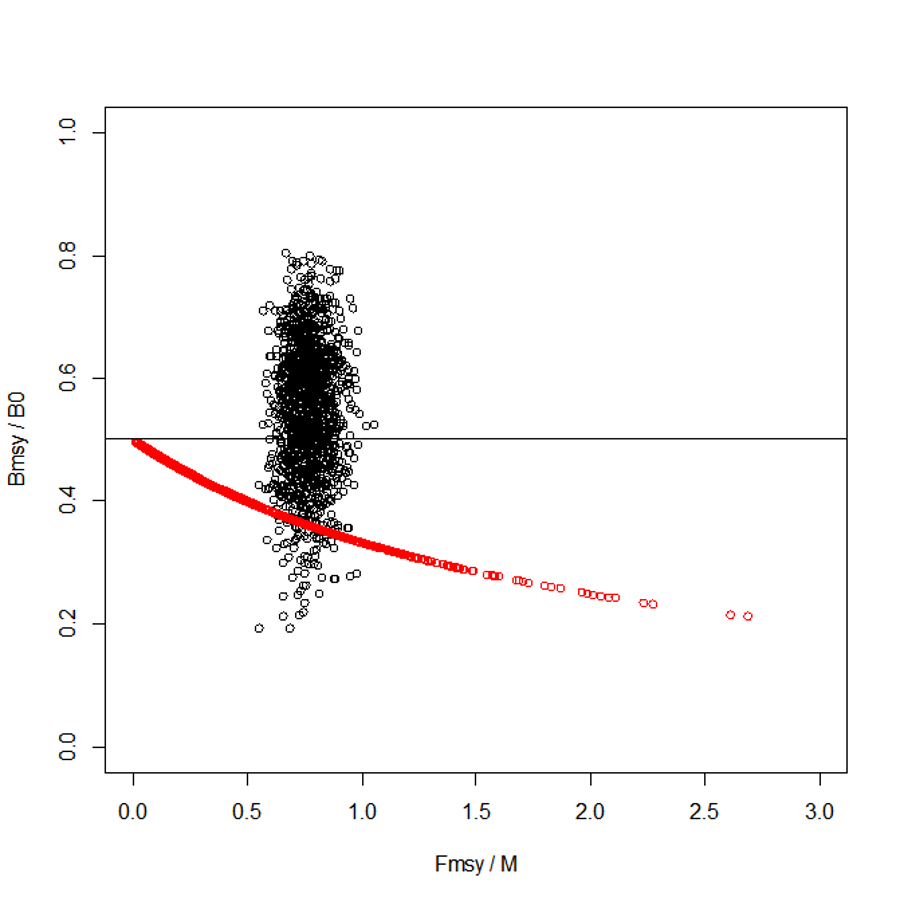
\includegraphics[width=1.4\textwidth]{cjasFig.png}
\end{minipage}
}
\only<2>{
\hspace*{-0.5cm}
\begin{minipage}[h!]{0.59\textwidth}
Conceptually:
\begin{align*}
\frac{F_{MSY}}{M}\in\mathbb{R}^+ ~~~ \frac{B_{MSY}}{B_{0}}\in\left(0, 1\right)
\end{align*}
$~$\\
Mangel et al. 2013, CJFAS:
\begin{itemize}
        \item BH Model: $~ \frac{F_{MSY}}{M}\in\mathbb{R}^+ ~~~ \frac{B_{MSY}}{\bar B(0)}=\frac{1}{F_{MSY}/M+2}$
        \item Similar Constraints for other Two-Parameter Curves %Logistic, Ricker and 
        \item Three-Parameter Relationships Allow Independent RP Estimation
\end{itemize}
\end{minipage}
\begin{minipage}[h!]{0.39\textwidth}
$~$\\
\hspace*{-0.3cm}
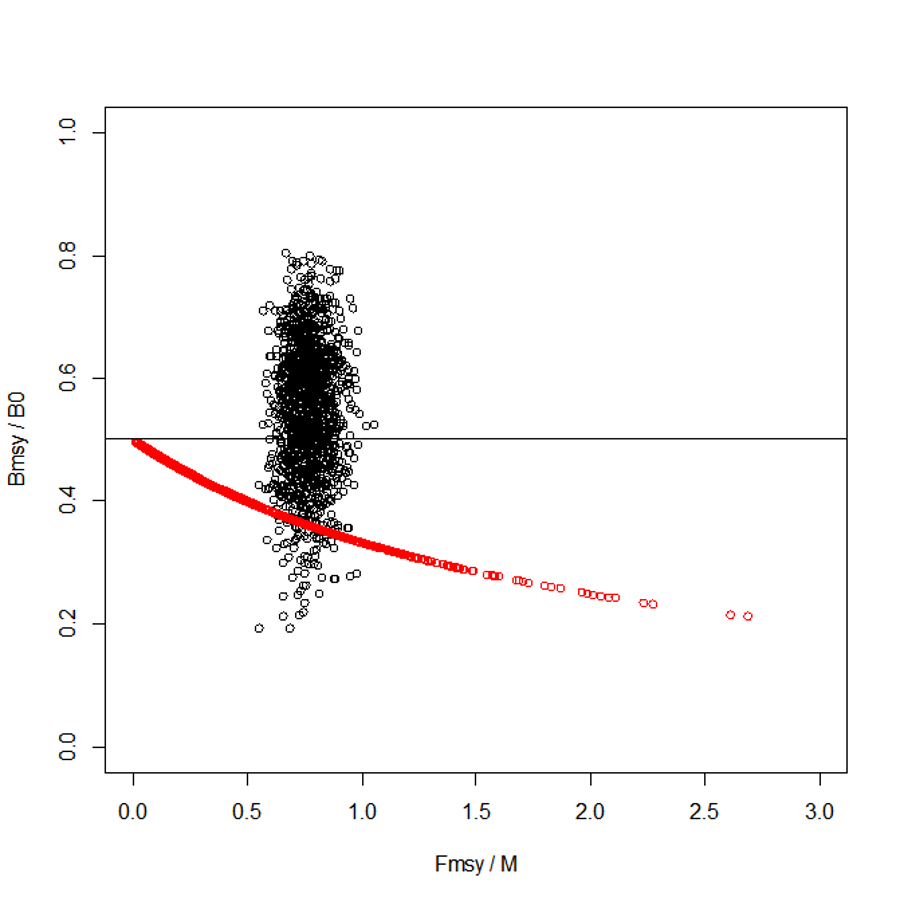
\includegraphics[width=1.4\textwidth]{cjasFig.png}
\end{minipage}
}
\end{frame}

%
\section{Simulation}
\subsection{}

%
\begin{frame}{Schnute 1985, CJFAS}
\begin{minipage}[h!]{0.49\textwidth}
\begin{align}
&\frac{dB}{dt} = P(B;\bm{\theta}) - (M+F)B \nonumber%\label{schunte}%
\end{align}
\begin{align}
&P(B;[\alpha, \beta, \gamma]) = \alpha B(1-\beta\gamma B)^{\frac{1}{\gamma}} \nonumber
\end{align}
\begin{align*}
\gamma = -1 &\Rightarrow \text{\color{ForestGreen}Beverton-Holt}\\
\gamma \rightarrow 0 &\Rightarrow \text{\color{RoyalBlue}Ricker}\\
\gamma = 1 &\Rightarrow  \text{\color{Red}Logistic}
\end{align*}
\end{minipage}
\begin{minipage}[h!]{0.49\textwidth}
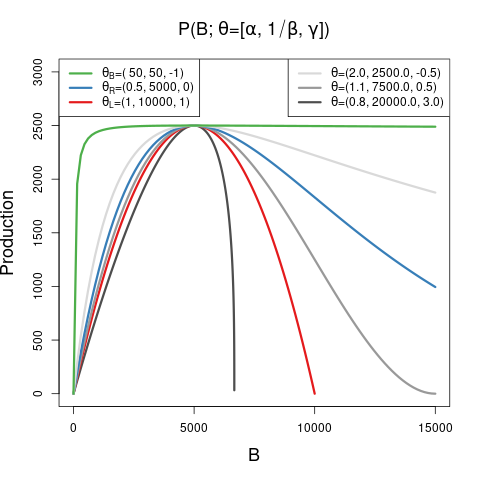
\includegraphics[width=1.1\textwidth]{./derisoSrr.png}
\end{minipage}
\end{frame}

%
\begin{frame}
\begin{minipage}[h!]{0.59\textwidth}
\begin{itemize}
\vspace{0.3cm}
\item Isolalting RP Bias is Hard:
\begin{itemize}
        \item Chaos in the Dynamical System
        \item Time Integrator Inaccuracy
        \item Model Identifiability
        \item Global Optimization
        \item etc...
\end{itemize}
\vspace{0.3cm}
\item Production Models are simplified places to build intuition % places to build from
\vspace{0.3cm}
%\item Build intuition relavant to Management 
\item See my analysis of the mechanisms of bias in the Schaefer Model $\Longrightarrow$
%that are useful for understanding toward 
%provide an intuitive modeling environment to build towards 
%\item Move towards
%\color{orange}
%%\item Starting from the rock bottom to build understanding
%\item And analysis of biases for the Scheaffer model can be seen here
%\item Schaefer Mechanistic Understanding
%%\item Attacking this problem from the ground up working towards age structred models is important due to the many computational issues that can arrise in ode modeling.
%%\begin{itemize}
%%	\item Chaos in the Dynamical System
%%	\item Time Integrator Inaccuracy
%%	\item Model Identifiability
%%	\item Global Optimization
%%	\item etc...
%%\end{itemize}
\end{itemize}
\end{minipage}
\begin{minipage}[h!]{0.39\textwidth}

\begin{center}
{\underline{\large Schaefer RP Analysis}}\\$~$\\
\href{https://ggle.io/5EnI}{
\includegraphics[height=0.5\textheight]{./talkQR.png}}\\$~$\\
\href{https://ggle.io/5EnI}{\color{blue}\texttt{https://ggle.io/5EnI}}
\end{center}

\end{minipage}
\end{frame}


%
\begin{frame}{Simulation Design}
\only<1>{
$~$\hspace{-1cm}
\begin{minipage}[h!]{0.59\textwidth}
\begin{itemize}
\item LHS design based on analytical results similar to Schnute and Richards 1998, CJFAS
\vspace{0.3cm}
\item[] % GP Metamodeling of RP bias
\vspace{0.6cm}
\end{itemize}
\begin{align*}
~\\~\\%\underbrace{\left(\frac{F_{MSY}}{M}, \frac{B_{MSY}}{\bar B(0)}\right)}_{\text{Schnute Truth}} {\text{GP}\atop{\mapsto\atop~}} \underbrace{\left(\frac{\hat F_{MSY}}{M}, \frac{\hat B_{MSY}}{\bar B(0)}\right)}_{\text{BH Estimate}}
\end{align*}
\end{minipage}
\begin{minipage}[h!]{0.39\textwidth}
\begin{center}
\begin{tikzpicture}[overlay]
\node at (1,0) {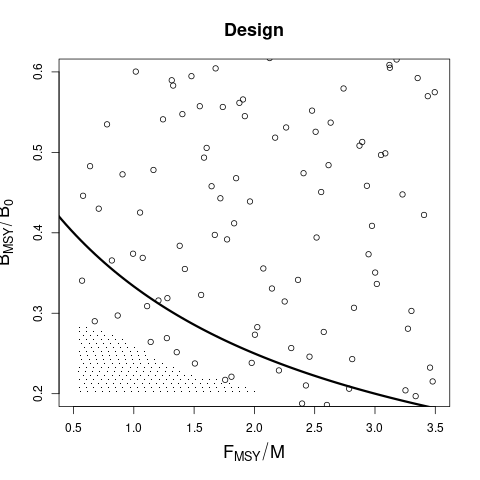
\includegraphics[height=0.7\textheight]{../gpBias/designLineHHardExpT45N150M0.3Wide.png}};
%\node[circle, draw, minimum size=7, inner sep=-2] at (2.6,1.5){\tiny S};
%\draw[latex-, very thick,black] (0.6,-0.9) -- ++(1.9,2.3);
%\node[circle,fill=red, minimum size=9, inner sep=-2] at (0.5,-1){\tiny BH};
\end{tikzpicture}
\end{center}
\end{minipage}
}
\only<2>{
$~$\hspace{-1cm}
\begin{minipage}[h!]{0.59\textwidth}
\begin{itemize}
\item LHS design based on analytical results similar to Schnute and Richards 1998, CJFAS
\vspace{0.3cm}
\item[] % GP Metamodeling of RP bias
\vspace{0.6cm}
\end{itemize}
\begin{align*}
~\\~\\%\underbrace{\left(\frac{F_{MSY}}{M}, \frac{B_{MSY}}{\bar B(0)}\right)}_{\text{Schnute Truth}} {\text{GP}\atop{\mapsto\atop~}} \underbrace{\left(\frac{\hat F_{MSY}}{M}, \frac{\hat B_{MSY}}{\bar B(0)}\right)}_{\text{BH Estimate}}
\end{align*}
\end{minipage}
\begin{minipage}[h!]{0.39\textwidth}
\begin{center}
\begin{tikzpicture}[overlay]
\node at (1,0) {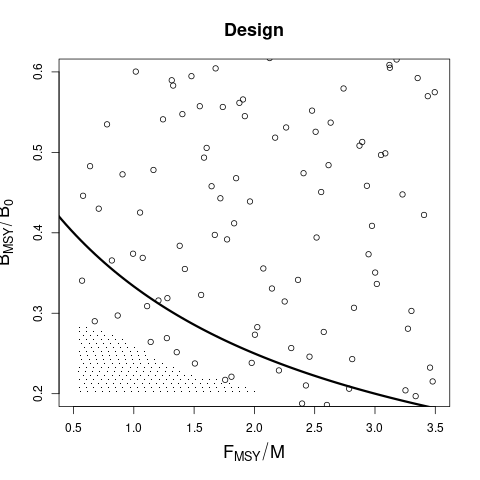
\includegraphics[height=0.7\textheight]{../gpBias/designLineHHardExpT45N150M0.3Wide.png}};
\node[circle, draw, minimum size=7, inner sep=-2] at (2.6,1.5){\tiny S};
\draw[latex-, very thick,black] (0.6,-0.9) -- ++(1.9,2.3);
\node[circle,fill=red, minimum size=9, inner sep=-2] at (0.5,-1){\tiny BH};
\end{tikzpicture}
\end{center}
\end{minipage}
}
\only<3>{
$~$\hspace{-1cm}
\begin{minipage}[h!]{0.59\textwidth}
\begin{itemize}
\item LHS design based on analytical results similar to Schnute and Richards 1998, CJFAS
\vspace{0.3cm}
\item GP Metamodeling of RP bias
\vspace{0.6cm}
\end{itemize}
\begin{equation*}
\underbrace{\left(\frac{F_{MSY}}{M}, \frac{B_{MSY}}{\bar B(0)}\right)}_{\text{Schnute Truth}} {\text{GP}\atop{\mapsto\atop~}} \underbrace{\left(\frac{\hat F_{MSY}}{M}, \frac{\hat B_{MSY}}{\bar B(0)}\right)}_{\text{BH Estimate}}
\end{equation*}
\end{minipage}
\begin{minipage}[h!]{0.39\textwidth}
\begin{center}
\begin{tikzpicture}[overlay]
\node at (1,0) {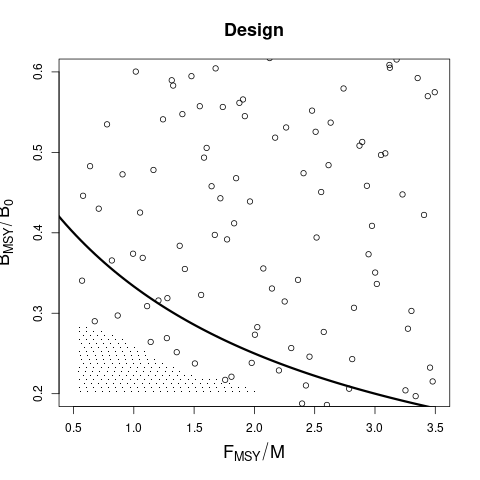
\includegraphics[height=0.7\textheight]{../gpBias/designLineHHardExpT45N150M0.3Wide.png}};
\node[circle, draw, minimum size=7, inner sep=-2] at (2.6,1.5){\tiny S};
\draw[latex-, very thick,black] (0.6,-0.9) -- ++(1.9,2.3);
\node[circle,fill=red, minimum size=9, inner sep=-2] at (0.5,-1){\tiny BH};
\end{tikzpicture}
\end{center}
\end{minipage}
}
\end{frame}

%
\begin{frame}{Catch}
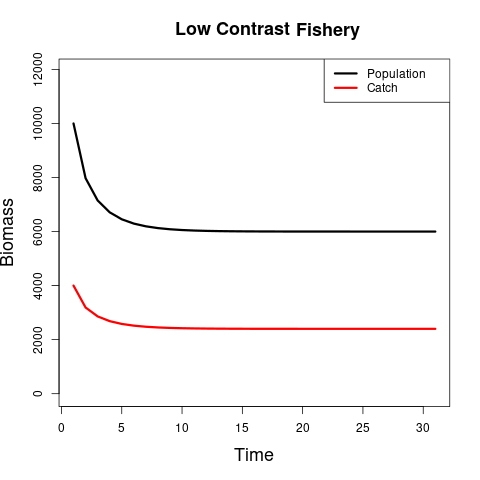
\includegraphics[width=0.49\textwidth]{../gpBias/bioCatchFlatNoQX2Z0.6NoPT.png}
%\hspace*{1cm}
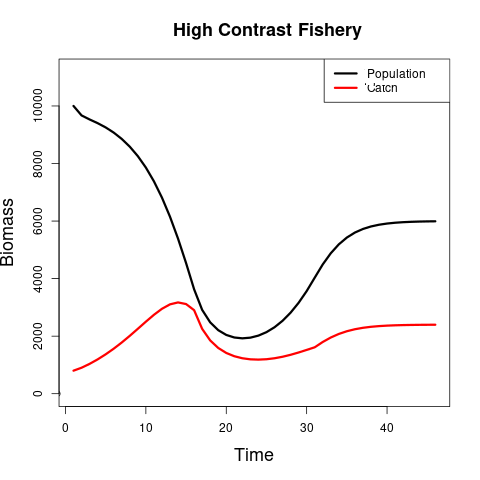
\includegraphics[width=0.49\textwidth]{../gpBias/bioCatchExpT45X2Z0.6NoPT.png}
\end{frame}

%
\section{Bias}
\subsection{}

%\begin{frame}{\color{orange}Results Idea List}
%\begin{itemize}
%\item contrast
%	\begin{itemize}
%		\item components
%		\item animated arrows and yeild curves
%	\end{itemize}
%\item flat
%\begin{itemize}
%	\item animated arrows and yeild curves
%\end{itemize}
%\end{itemize}
%\end{frame}

%%
%\begin{frame}%{Exp}
%%\vspace{-0.5cm}
%$~$
%\hspace*{-1.25cm}
%%\begin{minipage}[h!]{0.25\textwidth}
%%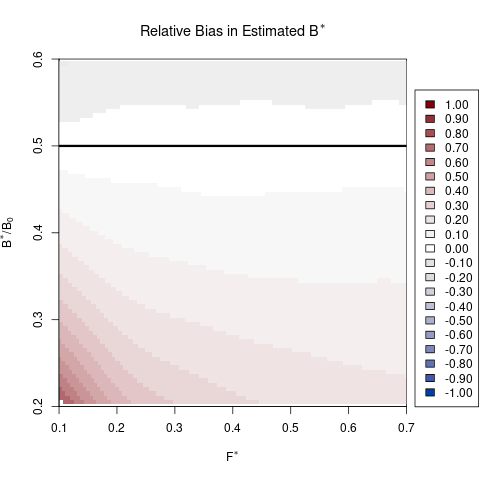
\includegraphics[width=1.1\textwidth]{~/Documents/school/ucscGrad/theses/nick/gpBias/bMSYRelBiasPellaExpNoQ.png}\\
%%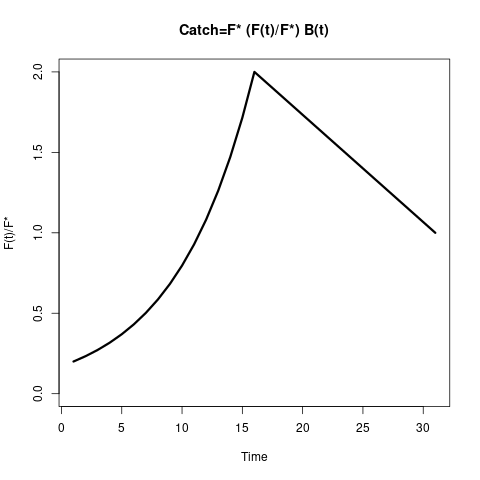
\includegraphics[width=1.1\textwidth]{~/Documents/school/ucscGrad/theses/nick/gpBias/catchExpNoQ.png}
%%\end{minipage}
%\begin{minipage}[h!]{0.33\textwidth}
%\hspace*{0.25cm}
%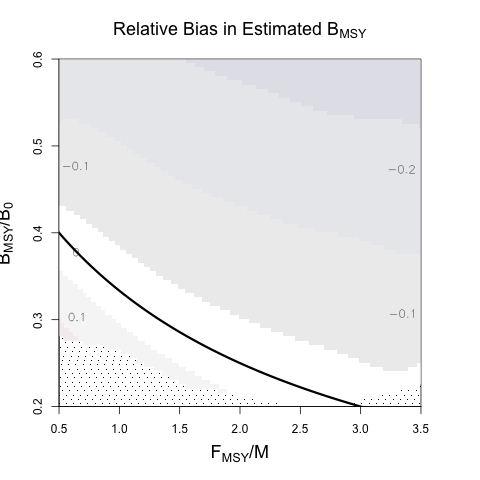
\includegraphics[width=1.1\textwidth]{../../../theses/nick/gpBias/bMSYRelBiasSchunteExpT45N150Wide.png}\\
%\hspace*{0.25cm}
%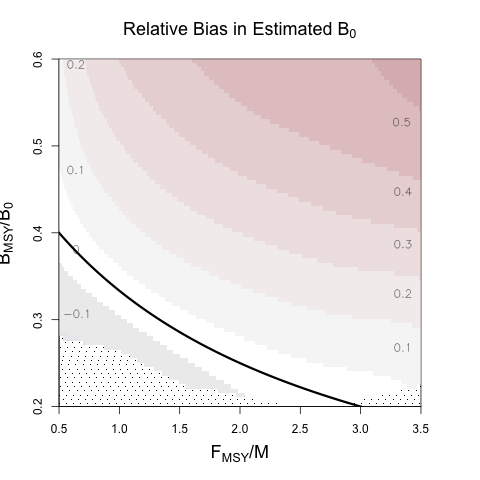
\includegraphics[width=1.1\textwidth]{../../../theses/nick/gpBias/kRelBiasSchnuteExpT45N150Wide.png}
%\end{minipage}
%\begin{minipage}[h!]{0.33\textwidth}
%\hspace*{0.75cm}
%%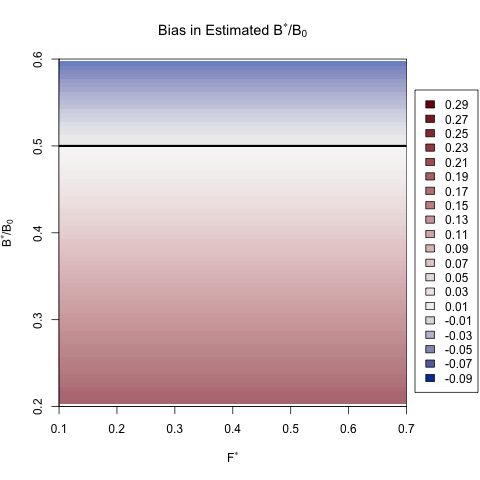
\includegraphics[width=1.1\textwidth]{../../../theses/nick/gpBias/zetaBiasPellaExpT45.png}\\
%%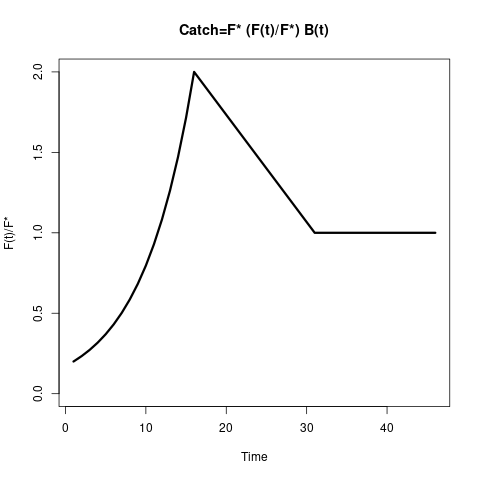
\includegraphics[width=1.1\textwidth]{../../../theses/nick/gpBias/catchExpT45.png}\\
%%\hspace*{0.75cm}
%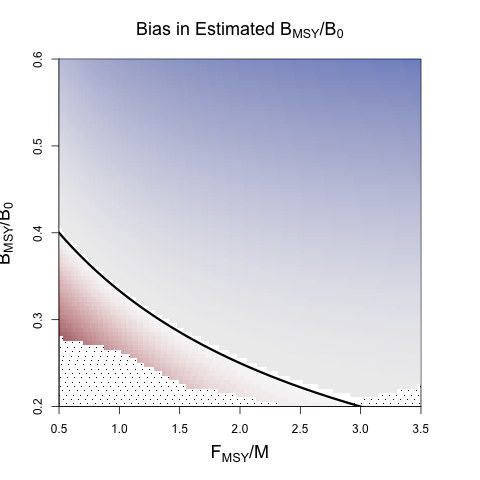
\includegraphics[width=1.1\textwidth]{../../../theses/nick/gpBias/zetaBiasSchnuteExpT45N150Wide.png}
%\end{minipage}
%\begin{minipage}[h!]{0.33\textwidth}
%%\hspace*{1cm}
%%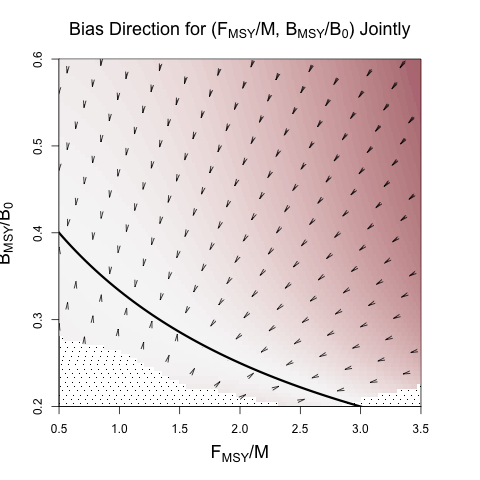
\includegraphics[width=1.1\textwidth]{../../../theses/nick/gpBias/directionalBiasSchnuteExpT45N150Wide.png}\\
%\hspace*{1cm}
%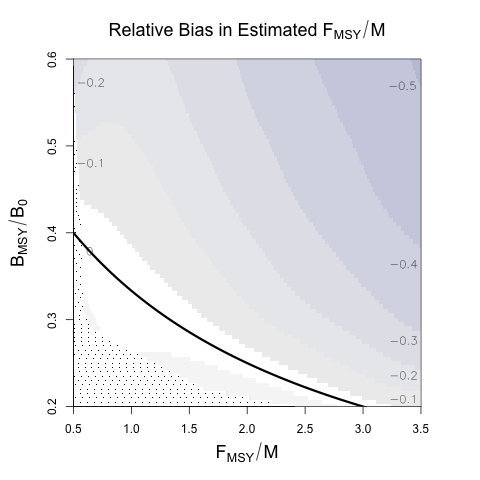
\includegraphics[width=1.1\textwidth]{../../../theses/nick/gpBias/fMSYRelBiasSchnuteExpT45N150Wide.png}
%\end{minipage}
%\end{frame}

%
\begin{frame}{High Contrast}
%\only<1>{
%\begin{center}
%\begin{tikzpicture}[overlay]
%	\node at (0,-0.5) {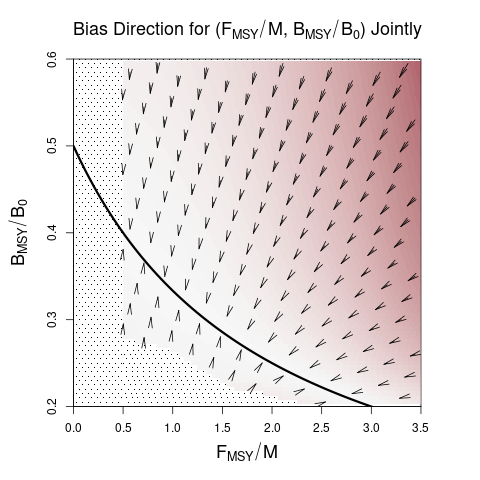
\includegraphics[height=1\textheight]{../gpBias/directionalBiasSchnuteAnimateBaseExpT45N150WideX3Z0.55.png}};
%	%\node at (4.5,2)  {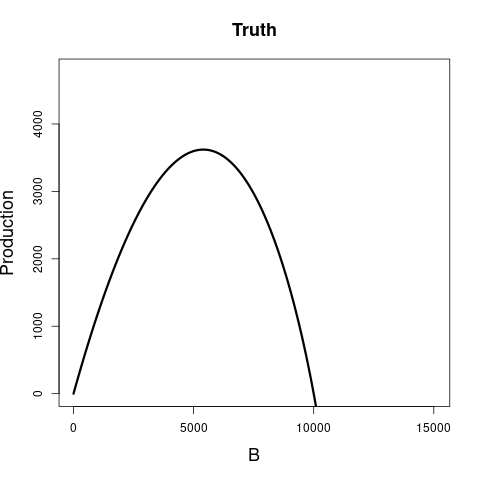
\includegraphics[scale=0.15]{../gpBias/yeildCurveTruthExpT45N150WideX3.348Z0.541.png}};
%	%\node at (-4.75,-2.5)  {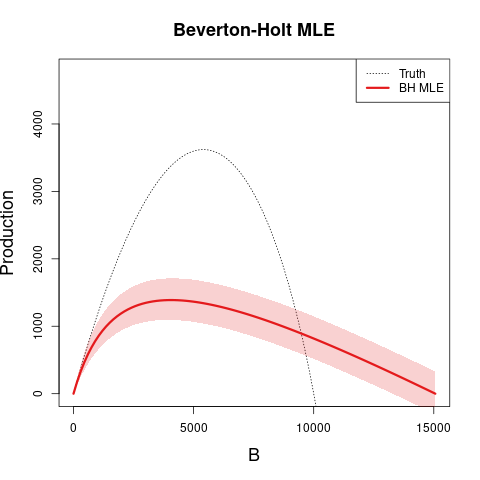
\includegraphics[scale=0.15]{../gpBias/yeildCurveFitExpT45N150WideX3.348Z0.541.png}};
%\end{tikzpicture}
%\end{center}
%}
%\only<2>{
%\begin{center}
%\begin{tikzpicture}[overlay]
%	\node at (0,-0.5) {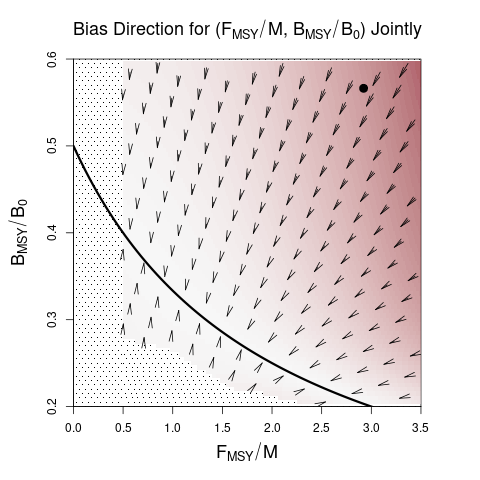
\includegraphics[height=1\textheight]{../gpBias/directionalBiasSchnuteAnimateSourceExpT45N150WideX3Z0.55.png}};
%	\node at (4.5,2)  {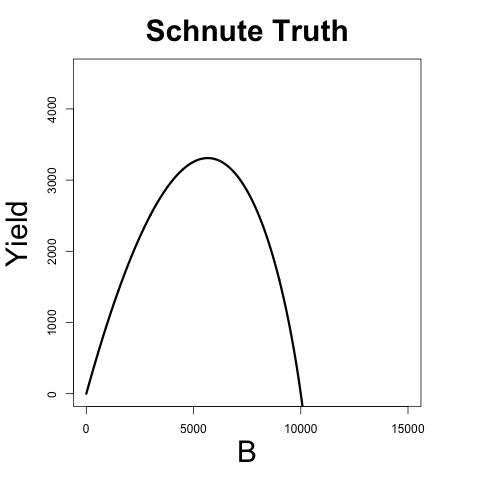
\includegraphics[scale=0.15]{../gpBias/yeildCurveTruthExpT45N150WideX3Z0.55.png}};
%	%\node at (-4.75,-2.5)  {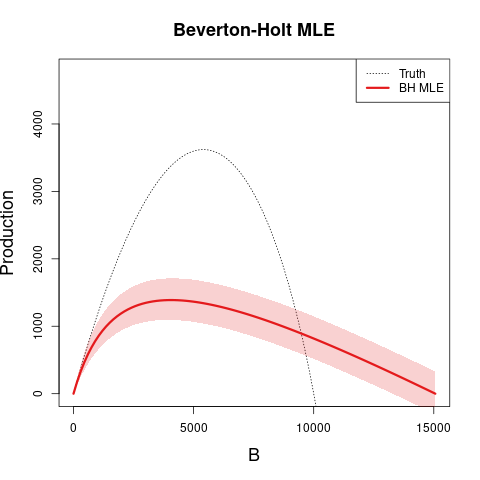
\includegraphics[scale=0.15]{../gpBias/yeildCurveFitExpT45N150WideX3.348Z0.541.png}};
%\end{tikzpicture}
%\end{center}
%}
%\only<3>{
%\begin{center}
%\begin{tikzpicture}[overlay]
%	\node at (0,-0.5) {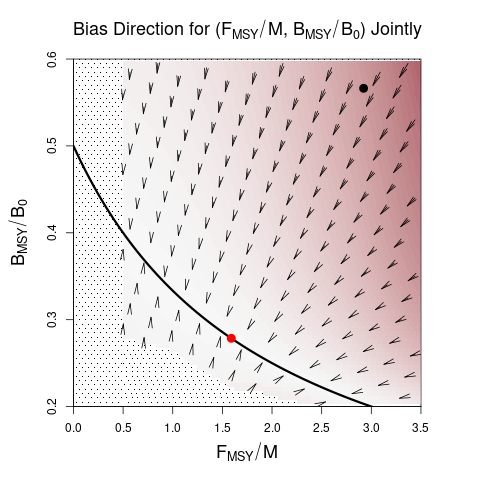
\includegraphics[height=1\textheight]{../gpBias/directionalBiasSchnuteAnimateSinkExpT45N150WideX3Z0.55.png}};
%	\node at (4.5,2)  {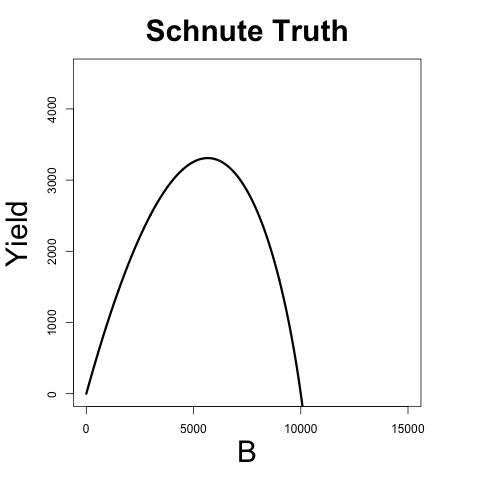
\includegraphics[scale=0.15]{../gpBias/yeildCurveTruthExpT45N150WideX3Z0.55.png}};
%	\node at (-4.75,-2.5)  {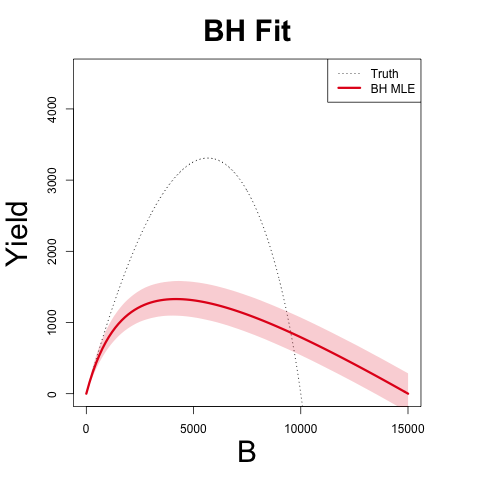
\includegraphics[scale=0.15]{../gpBias/yeildCurveFitExpT45N150WideX3Z0.55.png}};
%\end{tikzpicture}
%\end{center}
%}
\only<1>{
\begin{center}
\begin{tikzpicture}[overlay]                                                    
	\node at (0.25,-0.5) {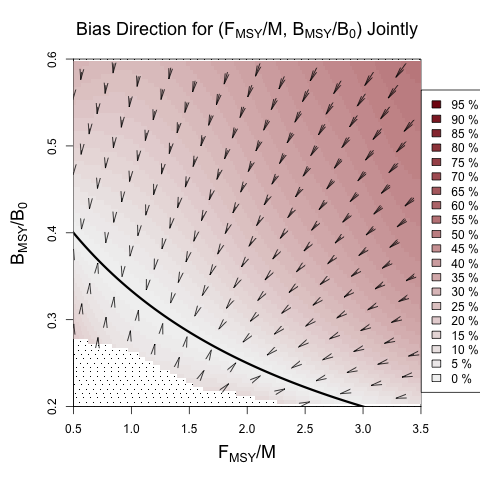
\includegraphics[height=0.92\textheight]{../gpBias/directionalBiasSchnuteAnimatePrecentExpT45N150WideX2.5Z0.45.png}};
	%\node at (4.5,2)  {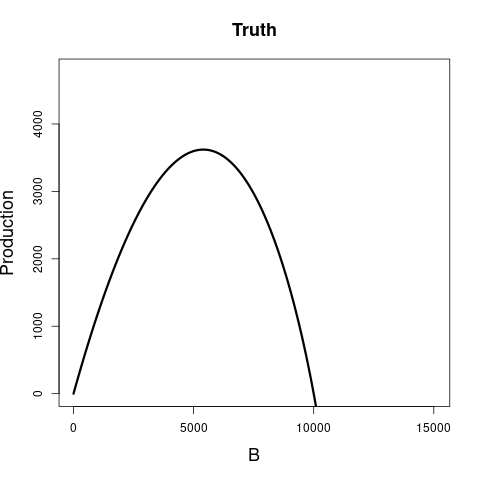
\includegraphics[scale=0.15]{../gpBias/yeildCurveTruthExpT45N150WideX3.348Z0.541.png}};
	%\node at (-4.75,-2.5)  {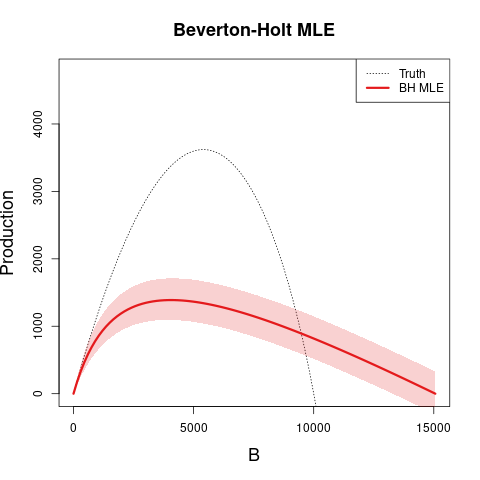
\includegraphics[scale=0.15]{../gpBias/yeildCurveFitExpT45N150WideX3.348Z0.541.png}};
\end{tikzpicture}
\end{center}
}
\only<2>{
\begin{center}
\begin{tikzpicture}[overlay]
	\node at (0.25,-0.5) {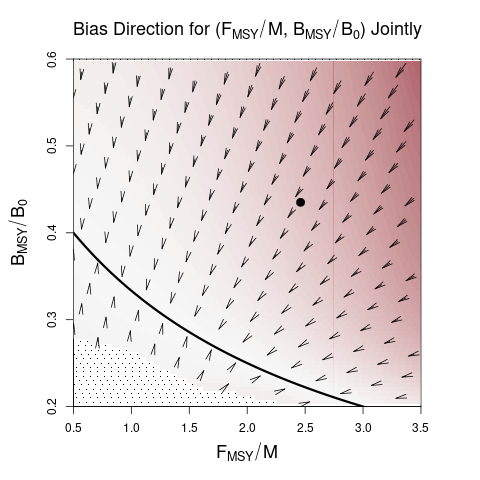
\includegraphics[height=0.92\textheight]{../gpBias/directionalBiasSchnuteAnimateSourceExpT45N150WideX2.5Z0.45.png}};
	\node at (4.75,0)  {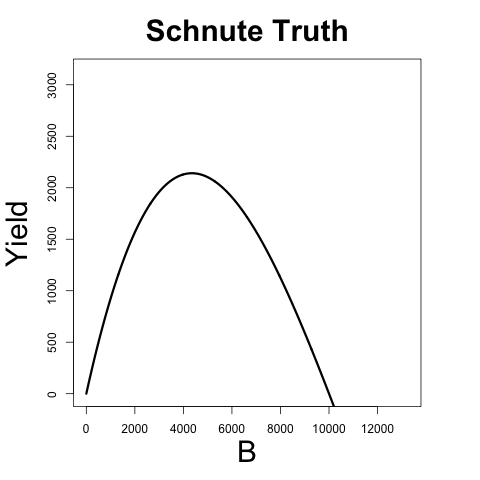
\includegraphics[scale=0.18]{../gpBias/yeildCurveTruthExpT45N150WideX2.5Z0.45.png}};
	%\node at (-4.75,-2.5)  {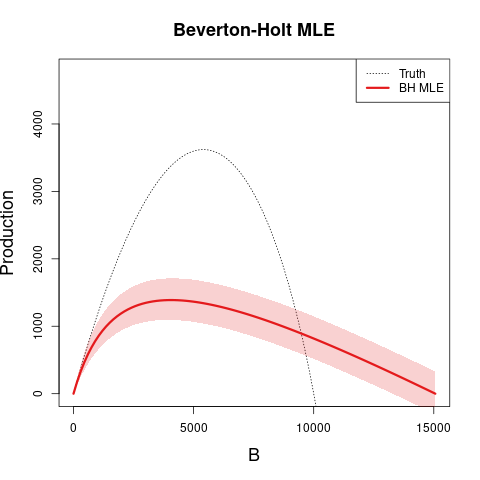
\includegraphics[scale=0.15]{../gpBias/yeildCurveFitExpT45N150WideX3.348Z0.541.png}};
\end{tikzpicture}
\end{center}
}
\only<3>{
\begin{center}
\begin{tikzpicture}[overlay]
	\node at (0.25,-0.5) {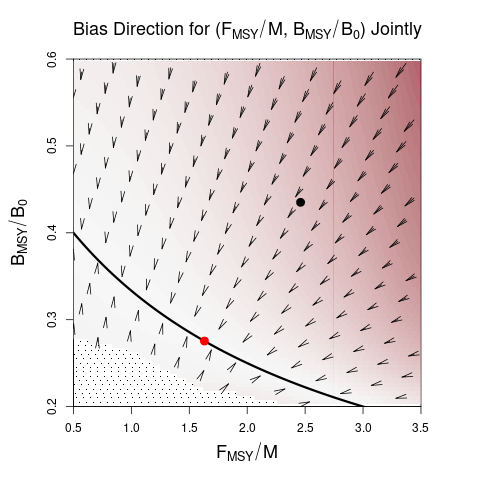
\includegraphics[height=0.92\textheight]{../gpBias/directionalBiasSchnuteAnimateSinkExpT45N150WideX2.5Z0.45.png}};
	\node at (4.75,0)  {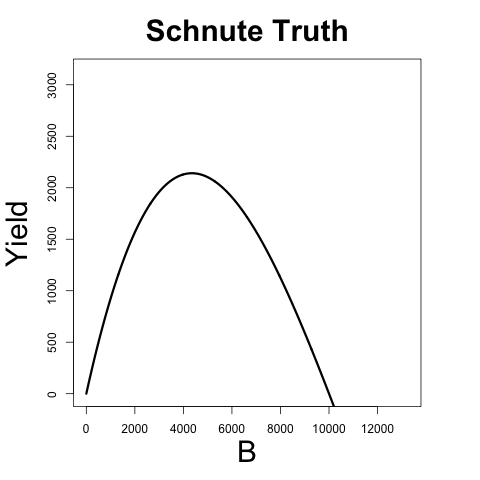
\includegraphics[scale=0.18]{../gpBias/yeildCurveTruthExpT45N150WideX2.5Z0.45.png}};
	\node at (-4.75,-2.25)  {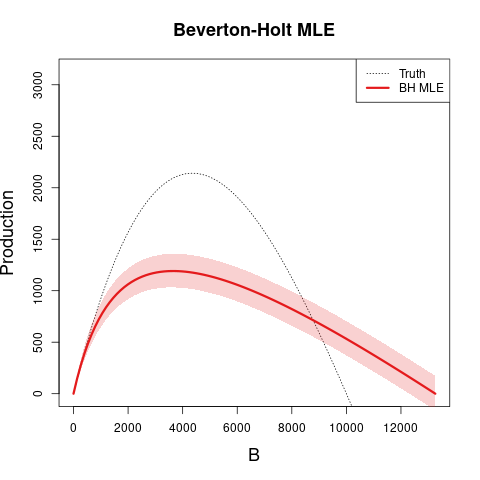
\includegraphics[scale=0.18]{../gpBias/yeildCurveFitExpT45N150WideX2.5Z0.45.png}};
\end{tikzpicture}
\end{center}
}
%\only<4>{
%\begin{center}
%\begin{tikzpicture}[overlay]
%	\node at (0.25,-0.5) {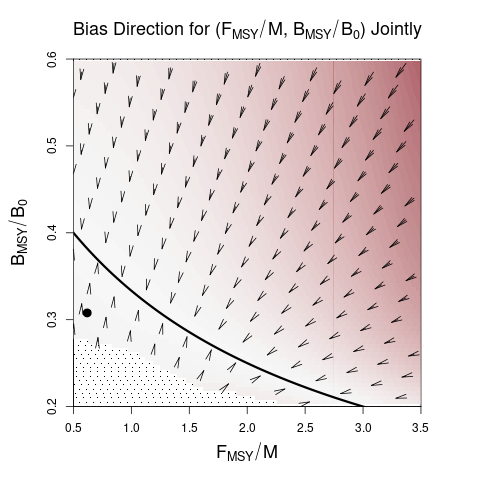
\includegraphics[height=0.92\textheight]{../gpBias/directionalBiasSchnuteAnimateSourceExpT45N150WideX0.5Z0.275.png}};
%	\node at (-4.75,-2.25)  {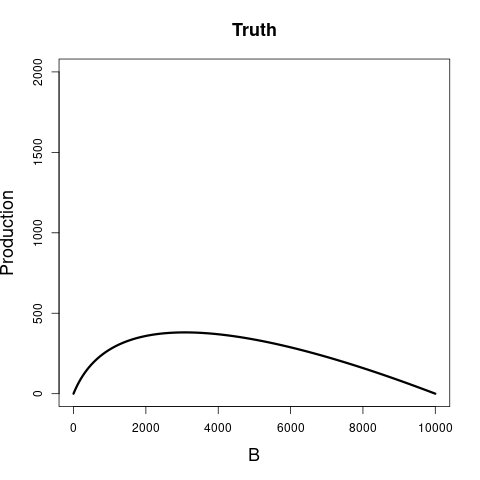
\includegraphics[scale=0.18]{../gpBias/yeildCurveTruthExpT45N150WideX0.5Z0.275.png}};
%	%\node at (-4.75,-2.5)  {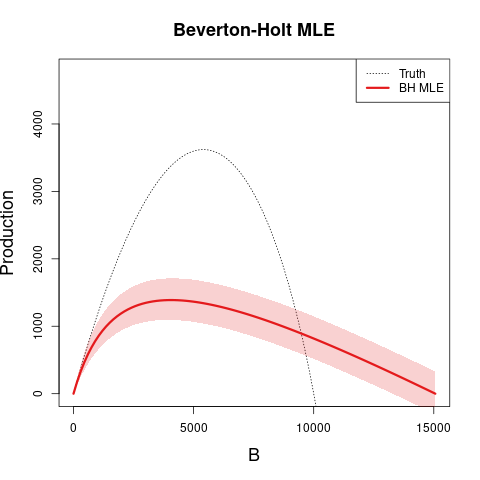
\includegraphics[scale=0.15]{../gpBias/yeildCurveFitExpT45N150WideX3.348Z0.541.png}};
%\end{tikzpicture}
%\end{center}
%}
%\only<5>{
%\begin{center}
%\begin{tikzpicture}[overlay]
%	\node at (0.25,-0.5) {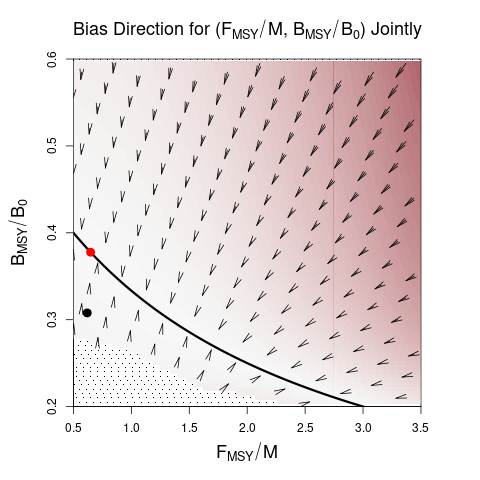
\includegraphics[height=0.92\textheight]{../gpBias/directionalBiasSchnuteAnimateSinkExpT45N150WideX0.5Z0.275.png}};
%	\node at (-4.75,-2.25)  {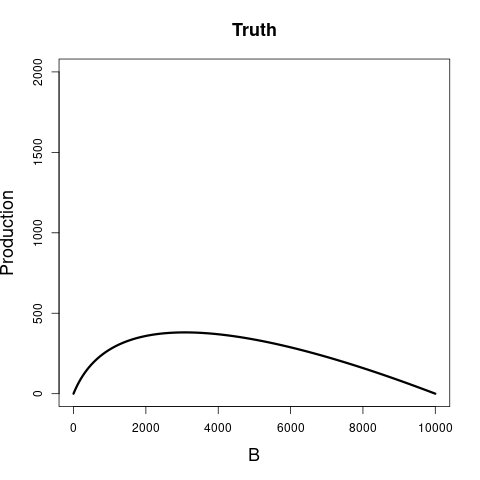
\includegraphics[scale=0.18]{../gpBias/yeildCurveTruthExpT45N150WideX0.5Z0.275.png}};
%	\node at (-4.75,1.5)  {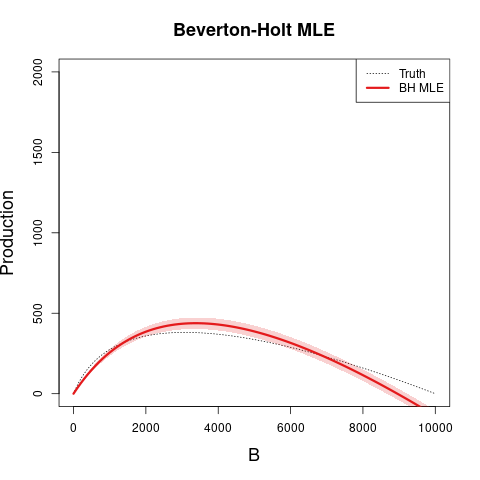
\includegraphics[scale=0.18]{../gpBias/yeildCurveFitExpT45N150WideX0.5Z0.275.png}};
%\end{tikzpicture}
%\end{center}
%}
%\only<6>{
%\begin{center}
%\begin{tikzpicture}[overlay]
%	\node at (0,-0.5) {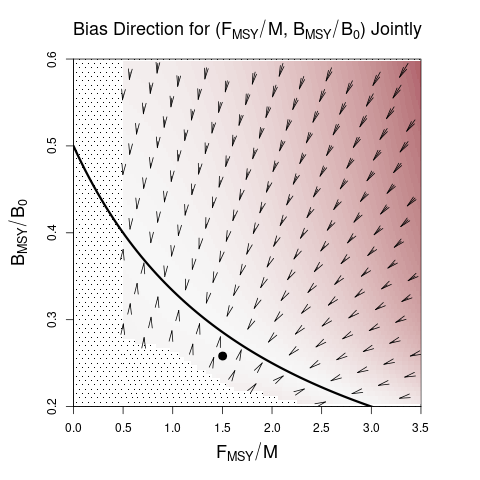
\includegraphics[height=0.92\textheight]{../gpBias/directionalBiasSchnuteAnimateSourceExpT45N150WideX1.5Z0.2.png}};
%	\node at (4.5,2)  {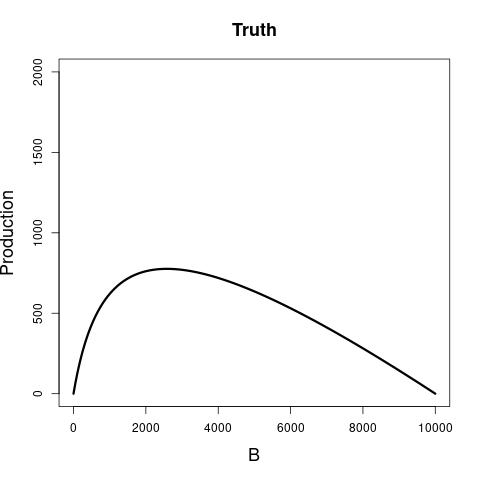
\includegraphics[scale=0.15]{../gpBias/yeildCurveTruthExpT45N150WideX1.5Z0.2.png}};
%	%\node at (-4.75,-2.5)  {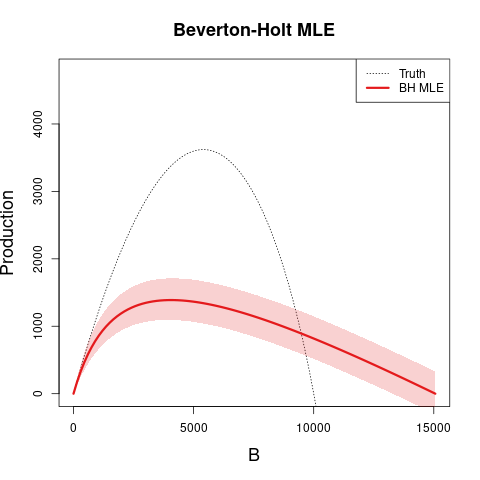
\includegraphics[scale=0.15]{../gpBias/yeildCurveFitExpT45N150WideX3.348Z0.541.png}};
%\end{tikzpicture}
%\end{center}
%}
%\only<7>{
%\begin{center}
%\begin{tikzpicture}[overlay]
%	\node at (0,-0.5) {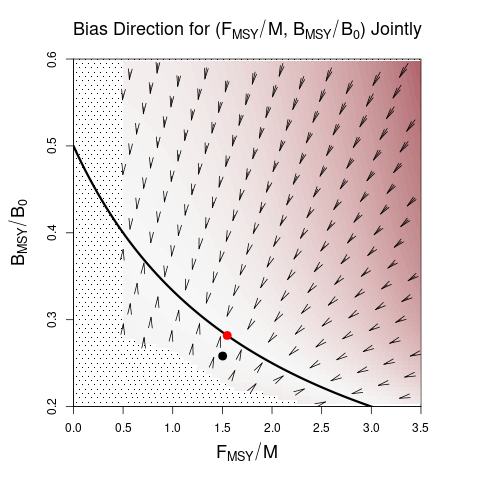
\includegraphics[height=0.92\textheight]{../gpBias/directionalBiasSchnuteAnimateSinkExpT45N150WideX1.5Z0.2.png}};
%	\node at (4.5,2)  {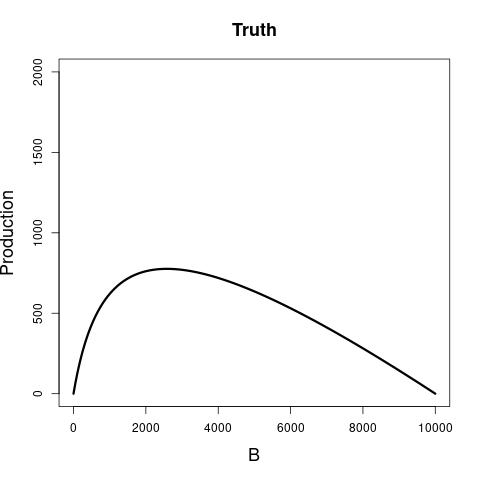
\includegraphics[scale=0.15]{../gpBias/yeildCurveTruthExpT45N150WideX1.5Z0.2.png}};
%	\node at (-4.75,-2.5)  {\includegraphics[scale=0.15]{../gpBias/yeildCurveFitExpT45N150WideX1.5Z0.2.png}};
%\end{tikzpicture}
%\end{center}
%}
%\only<8>{
%\begin{center}
%\begin{tikzpicture}[overlay]
%	\node at (0,-0.5) {\includegraphics[height=0.92\textheight]{../gpBias/directionalBiasSchnuteAnimateSourceExpT45N150WideX2Z0.2.png}};
%	\node at (4.5,2)  {\includegraphics[scale=0.15]{../gpBias/yeildCurveTruthExpT45N150WideX2Z0.2.png}};
%	%\node at (-4.75,-2.5)  {\includegraphics[scale=0.15]{../gpBias/yeildCurveFitExpT45N150WideX3.348Z0.541.png}};
%\end{tikzpicture}
%\end{center}
%}
%\only<9>{
%\begin{center}
%\begin{tikzpicture}[overlay]
%	\node at (0,-0.5) {\includegraphics[height=0.92\textheight]{../gpBias/directionalBiasSchnuteAnimateSinkExpT45N150WideX2Z0.2.png}};
%	\node at (4.5,2)  {\includegraphics[scale=0.15]{../gpBias/yeildCurveTruthExpT45N150WideX2Z0.2.png}};
%	\node at (-4.75,-2.5)  {\includegraphics[scale=0.15]{../gpBias/yeildCurveFitExpT45N150WideX2Z0.2.png}};
%\end{tikzpicture}
%\end{center}
%}
\end{frame}

%
\begin{frame}{Low Contrast}
\only<1>{
\begin{center}
\begin{tikzpicture}[overlay]
	\node at (0.25,-0.5) {\includegraphics[height=0.92\textheight]{../gpBias/directionalBiasSchnuteAnimatePrecentHHardFlatT30N150WWideN112X3Z0.55.png}};
	%\node at (4.5,2)  {\includegraphics[scale=0.15]{../gpBias/yeildCurveTruthHHardFlatT30N150WWideN56X3.497Z0.578.png}};
	%\node at (-4.75,-2.5)  {\includegraphics[scale=0.15]{../gpBias/yeildCurveFitHHardFlatT30N150WWideN56X3.497Z0.578.png}};
\end{tikzpicture}
\end{center}
}
\only<2>{
\begin{center}
\begin{tikzpicture}[overlay]
	\node at (0.25,-0.5) {\includegraphics[height=0.92\textheight]{../gpBias/directionalBiasSchnuteAnimateSourceHHardFlatT30N150WWideN112X3Z0.55.png}};
	\node at (4.75,1.5)  {\includegraphics[scale=0.18]{../gpBias/yeildCurveTruthHHardFlatT30N150WWideN112X3Z0.55.png}};
	%\node at (-4.75,-2.5)  {\includegraphics[scale=0.15]{../gpBias/yeildCurveFitHHardFlatT30N150WWideN56X3.497Z0.578.png}};
\end{tikzpicture}
\end{center}
}
\only<3>{
\begin{center}
\begin{tikzpicture}[overlay]
	\node at (0.25,-0.5) {\includegraphics[height=0.92\textheight]{../gpBias/directionalBiasSchnuteAnimateSinkHHardFlatT30N150WWideN112X3Z0.55.png}};
	\node at (4.75,1.5)  {\includegraphics[scale=0.18]{../gpBias/yeildCurveTruthHHardFlatT30N150WWideN112X3Z0.55.png}};
	\node at (-4.75,1.5)  {\includegraphics[scale=0.18]{../gpBias/yeildCurveFitHHardFlatT30N150WWideN112X3Z0.55.png}};
\end{tikzpicture}
\end{center}
}
%\only<4>{
%\begin{center}
%\begin{tikzpicture}[overlay]
%	\node at (0,-0.5) {\includegraphics[height=0.92\textheight]{../gpBias/directionalBiasSchnuteAnimateSourceHHardFlatT30N150WWideN56X3Z0.45.png}};
%	\node at (4.5,2)  {\includegraphics[scale=0.15]{../gpBias/yeildCurveTruthHHardFlatT30N150WWideN56X3Z0.45.png}};
%	%\node at (-4.75,-2.5)  {\includegraphics[scale=0.15]{../gpBias/yeildCurveFitHHardFlatT30N150WWideN56X3.497Z0.578.png}};
%\end{tikzpicture}
%\end{center}
%}
%\only<5>{
%\begin{center}
%\begin{tikzpicture}[overlay]
%	\node at (0,-0.5) {\includegraphics[height=0.92\textheight]{../gpBias/directionalBiasSchnuteAnimateSinkHHardFlatT30N150WWideN56X3Z0.45.png}};
%	\node at (4.5,2)  {\includegraphics[scale=0.15]{../gpBias/yeildCurveTruthHHardFlatT30N150WWideN56X3Z0.45.png}};
%	\node at (-4.75,-2.5)  {\includegraphics[scale=0.15]{../gpBias/yeildCurveFitHHardFlatT30N150WWideN56X3Z0.45.png}};
%\end{tikzpicture}
%\end{center}
%}
\only<4>{
\begin{center}
\begin{tikzpicture}[overlay]
	\node at (0.25,-0.5) {\includegraphics[height=0.92\textheight]{../gpBias/directionalBiasSchnuteAnimateSourceHHardFlatT30N150WWideN112X3Z0.35.png}};
	\node at (4.75,-1)  {\includegraphics[scale=0.18]{../gpBias/yeildCurveTruthHHardFlatT30N150WWideN112X3Z0.35.png}};
	%\node at (-4.75,-2.5)  {\includegraphics[scale=0.15]{../gpBias/yeildCurveFitHHardFlatT30N150WWideN56X3.497Z0.578.png}};
\end{tikzpicture}
\end{center}
}
\only<5>{
\begin{center}
\begin{tikzpicture}[overlay]
	\node at (0.25,-0.5) {\includegraphics[height=0.92\textheight]{../gpBias/directionalBiasSchnuteAnimateSinkHHardFlatT30N150WWideN112X3Z0.35.png}};
	\node at (4.75,-1)  {\includegraphics[scale=0.18]{../gpBias/yeildCurveTruthHHardFlatT30N150WWideN112X3Z0.35.png}};
	\node at (-4.75,-2.25)  {\includegraphics[scale=0.18]{../gpBias/yeildCurveFitHHardFlatT30N150WWideN112X3Z0.35.png}};
\end{tikzpicture}
\end{center}
}
\only<6>{
\begin{center}
\begin{tikzpicture}[overlay]
	\node at (0.25,-0.5) {\includegraphics[height=0.92\textheight]{../gpBias/directionalBiasSchnuteAnimateSinkHHardFlatT30N150WWideN112X3Z0.35.png}};
	\node at (4.75,-1)  {\includegraphics[scale=0.18]{../gpBias/yeildCurveTruthHHardFlatT30N150WWideN112X3Z0.35.png}};
	\node at (-4.75,-2.25)  {\includegraphics[scale=0.18]{../gpBias/yeildCurveFitHHardFlatT30N150WWideN112X3Z0.35.png}};
	\draw[very thick,blue] (-2.25,0.5) -- ++(5.25,-1.1);
\end{tikzpicture}
\end{center}
}
%\only<6>{
%\begin{center}
%\begin{tikzpicture}[overlay]
%	\node at (0,-0.5) {\includegraphics[height=0.92\textheight]{../gpBias/directionalBiasSchnuteAnimateSourceHHardFlatT30N150WWideN56X1Z0.275.png}};
%	\node at (4.5,2)  {\includegraphics[scale=0.15]{../gpBias/yeildCurveTruthHHardFlatT30N150WWideN56X1Z0.275.png}};
%	%\node at (-4.75,-2.5)  {\includegraphics[scale=0.15]{../gpBias/yeildCurveFitHHardFlatT30N150WWideN56X3.497Z0.578.png}};
%\end{tikzpicture}
%\end{center}
%}
%\only<7>{
%\begin{center}
%\begin{tikzpicture}[overlay]
%	\node at (0,-0.5) {\includegraphics[height=0.92\textheight]{../gpBias/directionalBiasSchnuteAnimateSinkHHardFlatT30N150WWideN56X1Z0.275.png}};
%	\node at (4.5,2)  {\includegraphics[scale=0.15]{../gpBias/yeildCurveTruthHHardFlatT30N150WWideN56X1Z0.275.png}};
%	\node at (-4.75,-2.5)  {\includegraphics[scale=0.15]{../gpBias/yeildCurveFitHHardFlatT30N150WWideN56X1Z0.275.png}};
%\end{tikzpicture}
%\end{center}
%}
\end{frame}

%
\section{End}
\subsection{}
%
\begin{frame}{Conclusions}
\begin{itemize}
	\setlength\itemsep{1em}
	\item A rich simulation-based method for describing global RP bias and a stepping stone for understanding more complex models.
	\begin{itemize}
                \item[$\Rightarrow$] Individual growth and maturity dynamics
        \end{itemize}
	\item RPs are not directly observable quantities, but rather model dependent latent quantities.
	\begin{itemize}
		\item[$\Rightarrow$] Subject to Model Misspecification, Uncertainty, \& Bias
		\item[$\Rightarrow$] In severly constrained settings we pay for our modeling mistakes primarily in estimate bias.
	\end{itemize}
	\item The observed contrast serves to increase the range of potentially ``allowable'' model misspecification. %distribute the available information among $B_{MSY}$ and $F_{MSY}$.
	%\item Importance of getting the computaional details correct for moving to analysis of Delay Difference and age structure
\end{itemize}
\end{frame}

%
\begin{frame}
\only<1>{
$~$\\$~$\\
\begin{minipage}[h!]{0.54\textwidth}
Many Thanks:\\
\begin{itemize}
\item UCSC Advisors
\item SWFSC Groundfish
\item NMFS Sea Grant
%\item Members of my Committee
\end{itemize}
\end{minipage}
\begin{minipage}[h!]{0.44\textwidth}
\includegraphics[width=0.9\textwidth]{rockFish.png}
\end{minipage}

%\vspace*{-0.5cm}
\begin{minipage}[h!]{0.59\textwidth}
\includegraphics[width=\textwidth]{seaGrant-logo.png}
\end{minipage}
\begin{minipage}[h!]{0.39\textwidth}
\includegraphics[width=\textwidth]{dssc.jpg}
\end{minipage}
}
\only<2>{
\frametitle{Metamodel Details}
\vspace*{-0.5cm}
\begin{align*}
        %\hat\mu &= \widehat{log(r)} ~~ -or- ~~ \hat\mu = \widehat{log(K)}\\
        %~\\
        \bm{x} &= \left(F_{MSY}, \frac{B_{MSY}}{\bar B(0)}\right) \nonumber\\
        ~\\
        \hat\mu &= \beta_0 + \bm{\beta}'\bm{x} + f(\bm{x}) + {\epsilon} \nonumber \\
        f(\bm{x}) &\sim \text{GP}(0, \tau^2 R(\bm{x}, \bm{x'})) \nonumber \\
        \epsilon_i &\sim \text{N}(0, \hat\omega_i).
\end{align*}
\begin{align*}
R(\bm{x}, \bm{x'}) &= \exp\left( \sum_{j=1}^2 \frac{-(x_j-x'_j)^2}{2\ell_j^2} \right)
\end{align*}
}
\only<3>{
\begin{center}
\includegraphics[width=0.7\textwidth]{../gpBias/crossCovExpT45.png}
\end{center}
}
\only<4>{
\frametitle{PT Data Fit with the Schaefer Model}
\begin{center}
 Low Contrast $~~~~~~~~~~~~~~~~~~~~~~$ High Contrast\\
\includegraphics[width=0.49\textwidth]{../gpBias/directionalBiasPellaFlatNoQ.png}
\includegraphics[width=0.49\textwidth]{../gpBias/directionalBiasPellaExpT45.png}
\end{center}
}
\only<5>{
\frametitle{Schnute RP-Parameter System of Equations}
\begin{align*}
\frac{B_{MSY}}{B_0} &= \frac{1-\left(\frac{M+F_{MSY}}{\alpha}\right)^\gamma}{ 1-\left(\frac{M}{\alpha}\right)^\gamma } \\
\alpha &= (M+F_{MSY})\left(1+\frac{\gamma F_{MSY}}{M+F_{MSY}}\right)^{1/\gamma} \\
\beta &= \frac{1}{\gamma B_0}\left(1-\left(\frac{M}{\alpha}\right)^\gamma\right)
\end{align*}
}
\only<6>{
\frametitle{Common Discretization}
\hspace*{-1cm}
\begin{minipage}[h!]{0.64\textwidth}
\begin{align*}
\frac{dB}{dt} &= P_\theta(B(t)) - C(t)
\end{align*}

\begin{align*}
%\frac{B(\tau+h)-B(\tau)}{h} &\approx h \left[P_\theta(B(\tau)) - C(\tau)\right]\\
B(\tau+1) &\approx B(\tau) + P_\theta(B(\tau)) - c(\tau)
\end{align*}
\end{minipage}
\begin{minipage}[h!]{0.24\textwidth}
\includegraphics[width=1.9\textwidth]{./eulerTry.png}
\end{minipage}
}
\end{frame}








%%
%\begin{frame}{\color{orange} Introish Ideas list}
%\begin{itemize}
%	\item PT/Schaffer work (link)
%	\item Computational Difficulties
%	\item {\color{orange}Schnute Space Filling}
%	\item Catch/Contrast
%\end{itemize}
%\end{frame}

%%
%\begin{frame}
%%
%\begin{minipage}[h!]{0.69\textwidth}
%%
%\begin{align*}
%\frac{B_{MSY}}{B_0} &= \frac{1-\left(\frac{M+F_{MSY}}{\alpha}\right)^\gamma}{ 1-\left(\frac{M}{\alpha}\right)^\gamma } \\
%\alpha &= (M+F_{MSY})\left(1+\frac{\gamma F_{MSY}}{M+F_{MSY}}\right)^{1/\gamma} \\
%\beta &= \frac{1}{\gamma B_0}\left(1-\left(\frac{M}{\alpha}\right)^\gamma\right)
%\end{align*}
%%
%\end{minipage}
%\begin{minipage}[h!]{0.29\textwidth}
%%
%\includegraphics[width=\textwidth]{../gpBias/designLineHHardExpT45N150M0.3Wide.png}
%\end{minipage}
%\end{frame}



%%
%\begin{frame}{\color{red}Catch}
%%
%\only<1>{
%\hspace*{-1cm}
%\begin{minipage}[h!]{0.24\textwidth}
%\begin{tikzpicture}
%  \node (img) {\includegraphics[width=1.1\textwidth]{../gpBias/catchFlat.png}};
%  %\draw[red, line width=1mm] 
%  %  (img.south west) -- (img.north east)
%  %  (img.south east) -- (img.north west);
%\end{tikzpicture}
%\end{minipage}
%\begin{minipage}[h!]{0.24\textwidth}
%$~$\\
%\hspace*{0.33cm}
%\begin{tikzpicture}
%  \node (img) {\includegraphics[width=1.1\textwidth]{../../../theses/nick/gpBias/catchCap.png}};
%  %\draw[red, line width=1mm] 
%  %  (img.south west) -- (img.north east)
%  %  (img.south east) -- (img.north west);
%\end{tikzpicture}
%\end{minipage}
%\begin{minipage}[h!]{0.24\textwidth}
%$~$\\
%\hspace*{0.66cm}
%\begin{tikzpicture}
%  \node (img) {\includegraphics[width=1.1\textwidth]{../../../theses/nick/gpBias/catchCupNoQ.png}};
%  %\draw[red, line width=1mm] 
%  %  (img.south west) -- (img.north east)
%  %  (img.south east) -- (img.north west);
%\end{tikzpicture}
%\end{minipage}
%\begin{minipage}[h!]{0.24\textwidth}
%$~$\\
%\hspace*{1cm}
%\begin{tikzpicture}
%  \node (img) {\includegraphics[width=1.1\textwidth]{../../../theses/nick/gpBias/catchExp.png}};
%  %\draw[red, line width=1mm] 
%  %  (img.south west) -- (img.north east)
%  %  (img.south east) -- (img.north west);
%\end{tikzpicture}
%\end{minipage}
%%\end{frame}
%}
%%
%%\begin{frame}{Catch}
%\only<2>{
%%
%\vspace*{-0.3cm}
%\hspace*{-1cm}
%\begin{minipage}[h!]{0.24\textwidth}
%\begin{tikzpicture}
%  \node[below] (img) at (0, 2.5) {};
%  \node (img) {\includegraphics[width=1.1\textwidth]{../../../theses/nick/gpBias/catchFlat.png}};
%  \node[above] (img) at (0, -2.5) {Flat};
%  %\draw[red, line width=1mm] 
%  %  (img.south west) -- (img.north east)
%  %  (img.south east) -- (img.north west);
%\end{tikzpicture}
%\end{minipage}
%\begin{minipage}[h!]{0.24\textwidth}
%$~$\\
%\hspace*{0.33cm}
%\begin{tikzpicture}
%  \node (img) {\includegraphics[width=1.1\textwidth]{../../../theses/nick/gpBias/catchCap.png}};
%  \draw[red, line width=1mm] 
%    (img.south west) -- (img.north east)
%    (img.south east) -- (img.north west);
%\end{tikzpicture}
%\end{minipage}
%\begin{minipage}[h!]{0.24\textwidth}
%$~$\\
%\hspace*{0.66cm}
%\begin{tikzpicture}
%  \node (img) {\includegraphics[width=1.1\textwidth]{../../../theses/nick/gpBias/catchCupNoQ.png}};
%  \draw[red, line width=1mm] 
%    (img.south west) -- (img.north east)
%    (img.south east) -- (img.north west);
%\end{tikzpicture}
%\end{minipage}
%\begin{minipage}[h!]{0.24\textwidth}
%$~$\\
%\hspace*{1cm}
%\begin{tikzpicture}
%  \node[below] (img) at (0, 2.5) {};
%  \node (img) {\includegraphics[width=1.1\textwidth]{../../../theses/nick/gpBias/catchExp.png}};
%  \node[above] (img) at (0, -2.5) {Contrast};
%  %\draw[red, line width=1mm] 
%  %  (img.south west) -- (img.north east)
%  %  (img.south east) -- (img.north west);
%\end{tikzpicture}
%\end{minipage}
%}
%\end{frame}

%%%
%%\begin{frame}{Catch}
%%%\begin{itemize}
%%%\item catch parameterization
%%%\item implied index shapes
%%%\item continuity
%%%\end{itemize}
%%\includegraphics[width=0.24\textwidth]{~/Documents/school/ucscGrad/theses/nick/gpBias/catchFlat.png}
%%\includegraphics[width=0.24\textwidth]{~/Documents/school/ucscGrad/theses/nick/gpBias/catchCap.png}
%%\includegraphics[width=0.24\textwidth]{~/Documents/school/ucscGrad/theses/nick/gpBias/catchCupNoQ.png}
%%\includegraphics[width=0.24\textwidth]{~/Documents/school/ucscGrad/theses/nick/gpBias/catchExp.png}
%%\end{frame}
%
%
%%\includegraphics[width=0.24\textwidth]{~/Documents/school/ucscGrad/theses/nick/gpBias/catchFlat.png}
%%\includegraphics[width=0.24\textwidth]{~/Documents/school/ucscGrad/theses/nick/gpBias/catchCap.png}
%%\includegraphics[width=0.24\textwidth]{~/Documents/school/ucscGrad/theses/nick/gpBias/catchCupNoQ.png}
%%\includegraphics[width=0.24\textwidth]{~/Documents/school/ucscGrad/theses/nick/gpBias/catchExp.png}
%%\begin{itemize}
%%\item catch parameterization
%%\item implied index shapes
%%\item continuity
%%\end{itemize}
%
%%\section{Methods}
%%\subsection{}



%{
%\color{gray}
%%
%\begin{frame}{Pella-Tomlinson Production Model}
%\only<1>{
%\vspace{-0.6cm}
%\hspace*{-1cm}
%\begin{minipage}[h!]{0.55\textwidth}
%\begin{align*}
%	I(t) &\sim LN(qB(t), \sigma^2)\\
%	\frac{dB(t)}{dt} &= R_{\bm{\theta}}(B(t)) - F(t)B(t)\\
%	R_{\bm{\theta}}(B) &= \frac{rB}{\gamma-1} \left(1-\frac{B}{K}\right)^{\gamma-1}\\
%	\bm{\theta} &= (r, K, \gamma)\\
%	~&~\\
%	\gamma &= 2 \Rightarrow \text{Schaefer Model}
%\end{align*}
%\end{minipage}
%\begin{minipage}[h!]{0.45\textwidth}
%%\includegraphics[width=\textwidth]{~../../../theses/nick/gpBias/srrSchaeffer.png}
%\includegraphics[width=1.2\textwidth]{srrSchaeffer.png}
%\end{minipage}
%}
%
%%\begin{frame}{Pella-Tomlinson Production Model}
%\only<2>{
%\vspace{-0.6cm}
%\hspace*{-1cm}
%\begin{minipage}[h!]{0.55\textwidth}
%\begin{align*}
%	I(t) &\sim LN(qB(t), \sigma^2)\\
%	\frac{dB(t)}{dt} &= R_{\bm{\theta}}(B(t)) - F(t)B(t)\\
%	R_{\bm{\theta}}(B) &= \frac{rB}{\gamma-1} \left(1-\frac{B}{K}\right)^{\gamma-1}\\
%	\bm{\theta} &= (r, K, \gamma)\\
%	~&~\\
%	\gamma &= 2 \Rightarrow \text{Schaefer Model}
%\end{align*}
%\end{minipage}
%\begin{minipage}[h!]{0.45\textwidth}
%%\includegraphics[width=\textwidth]{~../../../theses/nick/gpBias/srrSchaeffer.png}
%\includegraphics[width=1.2\textwidth]{shaeferConst.png}
%\end{minipage}
%}
%\end{frame}
%
%%
%\begin{frame}{Pella-Tomlinson Family of Curves}
%%\begin{itemize}
%%\item Pella-Tomlinson Shapes
%%\item Restriction to Schaffer
%%\end{itemize}
%\includegraphics[width=0.49\textwidth]{srr1.1.png}
%\includegraphics[width=0.49\textwidth]{srr2.png}
%%$~~$ Beverton-Holt $~~~~~~~~~~~$ Shaefer (logistic) $~~~~~~~~~~~~~$ Schunte\\
%%\mbox{$~~~R(B) = \frac{\alpha B}{1+\beta B}~~~~~~~~~~R(B) = \alpha B (1-\beta B)~~~~R(B) = \alpha B (1-\beta\gamma B)^{\frac{1}{\gamma}}$}\\
%%\hspace*{-0.7cm}
%%\includegraphics[width=0.38\textwidth]{../bh.jpg}
%%\includegraphics[width=0.38\textwidth]{../sha.jpg}
%%\includegraphics[width=0.38\textwidth]{../der.jpg}
%\end{frame}
%
%%
%\begin{frame}
%\begin{center}
%\includegraphics[height=1\textheight]{shaeferDat.png}
%\end{center}
%\end{frame}
%}


%{
%\color{gray}
%%
%\begin{frame}%{Flat}
%%\vspace{-0.5cm}
%$~$
%\vspace*{-0.5cm}
%\hspace*{-1.25cm}
%%\begin{minipage}[h!]{0.25\textwidth}
%%\includegraphics[width=1.1\textwidth]{~/Documents/school/ucscGrad/theses/nick/gpBias/bMSYRelBiasPellaFlatNoQ.png}\\
%%\includegraphics[width=1.1\textwidth]{~/Documents/school/ucscGrad/theses/nick/gpBias/catchFlatNoQ.png}
%%\end{minipage}
%\begin{minipage}[h!]{0.33\textwidth}
%\hspace*{0.25cm}
%\includegraphics[width=1.1\textwidth]{../../../theses/nick/gpBias/bMSYRelBiasPellaFlatNoQ.png}\\
%\hspace*{0.25cm}
%\includegraphics[width=1.1\textwidth]{../../../theses/nick/gpBias/kRelBiasPellaFlatNoQ.png}
%\end{minipage}
%\begin{minipage}[h!]{0.33\textwidth}
%\hspace*{0.75cm}
%%\includegraphics[width=1.1\textwidth]{../../../theses/nick/gpBias/zetaBiasPellaFlatNoQ.png}\\
%\includegraphics[width=1.1\textwidth]{../../../theses/nick/gpBias/catchFlat.png}\\
%\hspace*{0.75cm}
%\includegraphics[width=1.1\textwidth]{../../../theses/nick/gpBias/msyRelBiasPellaFlatNoQ.png}
%\end{minipage}
%\begin{minipage}[h!]{0.33\textwidth}
%\hspace*{1cm}
%\includegraphics[width=1.1\textwidth]{../../../theses/nick/gpBias/directionalBiasPellaFlatNoQ.png}\\
%\hspace*{1cm}
%\includegraphics[width=1.1\textwidth]{../../../theses/nick/gpBias/fMSYRelBiasPellaFlatNoQ.png}
%\end{minipage}
%\end{frame}
%
%%%
%%\begin{frame}%{Flat}
%%%\vspace{-0.5cm}
%%$~$
%%\vspace*{-0.5cm}
%%\hspace*{-1.25cm}
%%%\begin{minipage}[h!]{0.25\textwidth}
%%%\includegraphics[width=1.1\textwidth]{~/Documents/school/ucscGrad/theses/nick/gpBias/bMSYRelBiasPellaFlatNoQ.png}\\
%%%\includegraphics[width=1.1\textwidth]{~/Documents/school/ucscGrad/theses/nick/gpBias/catchFlatNoQ.png}
%%%\end{minipage}
%%\begin{minipage}[h!]{0.33\textwidth}
%%\hspace*{0.25cm}
%%\includegraphics[width=1.1\textwidth]{../../../theses/nick/gpBias/bMSYRelBiasPellaFlatT35.png}\\
%%\hspace*{0.25cm}
%%\includegraphics[width=1.1\textwidth]{../../../theses/nick/gpBias/kRelBiasPellaFlatT35.png}
%%\end{minipage}
%%\begin{minipage}[h!]{0.33\textwidth}
%%\hspace*{0.75cm}
%%\includegraphics[width=1.1\textwidth]{../../../theses/nick/gpBias/zetaBiasPellaFlatT35.png}\\
%%\hspace*{0.75cm}
%%\includegraphics[width=1.1\textwidth]{../../../theses/nick/gpBias/catchFlatT35.png}
%%\end{minipage}
%%\begin{minipage}[h!]{0.33\textwidth}
%%\hspace*{1cm}
%%\includegraphics[width=1.1\textwidth]{../../../theses/nick/gpBias/directionalBiasPellaFlatT35.png}\\
%%\hspace*{1cm}
%%\includegraphics[width=1.1\textwidth]{../../../theses/nick/gpBias/fMSYRelBiasPellaFlatT35.png}
%%\end{minipage}
%%\end{frame}
%
%%
%\begin{frame}%{Exp}
%%\vspace{-0.5cm}
%$~$
%\hspace*{-1.25cm}
%%\begin{minipage}[h!]{0.25\textwidth}
%%\includegraphics[width=1.1\textwidth]{~/Documents/school/ucscGrad/theses/nick/gpBias/bMSYRelBiasPellaExpNoQ.png}\\
%%\includegraphics[width=1.1\textwidth]{~/Documents/school/ucscGrad/theses/nick/gpBias/catchExpNoQ.png}
%%\end{minipage}
%\begin{minipage}[h!]{0.33\textwidth}
%\hspace*{0.25cm}
%\includegraphics[width=1.1\textwidth]{../../../theses/nick/gpBias/bMSYRelBiasPellaExpNoQ.png}\\
%\hspace*{0.25cm}
%\includegraphics[width=1.1\textwidth]{../../../theses/nick/gpBias/kRelBiasPellaExpNoQ.png}
%\end{minipage}
%\begin{minipage}[h!]{0.33\textwidth}
%\hspace*{0.75cm}
%%\includegraphics[width=1.1\textwidth]{../../../theses/nick/gpBias/zetaBiasPellaExpNoQ.png}\\
%\includegraphics[width=1.1\textwidth]{../../../theses/nick/gpBias/catchExp.png}\\
%\hspace*{0.75cm}
%\includegraphics[width=1.1\textwidth]{../../../theses/nick/gpBias/msyRelBiasPellaExpNoQ.png}
%\end{minipage}
%\begin{minipage}[h!]{0.33\textwidth}
%\hspace*{1cm}
%\includegraphics[width=1.1\textwidth]{../../../theses/nick/gpBias/directionalBiasPellaExpNoQ.png}\\
%\hspace*{1cm}
%\includegraphics[width=1.1\textwidth]{../../../theses/nick/gpBias/fMSYRelBiasPellaExpNoQ.png}
%\end{minipage}
%\end{frame}
%
%%
%\begin{frame}%{Exp}
%%\vspace{-0.5cm}
%$~$
%\hspace*{-1.25cm}
%%\begin{minipage}[h!]{0.25\textwidth}
%%\includegraphics[width=1.1\textwidth]{~/Documents/school/ucscGrad/theses/nick/gpBias/bMSYRelBiasPellaExpNoQ.png}\\
%%\includegraphics[width=1.1\textwidth]{~/Documents/school/ucscGrad/theses/nick/gpBias/catchExpNoQ.png}
%%\end{minipage}
%\begin{minipage}[h!]{0.33\textwidth}
%\hspace*{0.25cm}
%\includegraphics[width=1.1\textwidth]{../../../theses/nick/gpBias/bMSYRelBiasPellaExpT45.png}\\
%\hspace*{0.25cm}
%\includegraphics[width=1.1\textwidth]{../../../theses/nick/gpBias/kRelBiasPellaExpT45.png}
%\end{minipage}
%\begin{minipage}[h!]{0.33\textwidth}
%\hspace*{0.75cm}
%%\includegraphics[width=1.1\textwidth]{../../../theses/nick/gpBias/zetaBiasPellaExpT45.png}\\
%\includegraphics[width=1.1\textwidth]{../../../theses/nick/gpBias/catchExpT45.png}\\
%\hspace*{0.75cm}
%\includegraphics[width=1.1\textwidth]{../../../theses/nick/gpBias/msyRelBiasPellaExpT45.png}
%\end{minipage}
%\begin{minipage}[h!]{0.33\textwidth}
%\hspace*{1cm}
%\includegraphics[width=1.1\textwidth]{../../../theses/nick/gpBias/directionalBiasPellaExpT45.png}\\
%\hspace*{1cm}
%\includegraphics[width=1.1\textwidth]{../../../theses/nick/gpBias/fMSYRelBiasPellaExpT45.png}
%\end{minipage}
%\end{frame}
%
%%
%\begin{frame}%{Exp}
%%\vspace{-0.5cm}
%$~$
%\hspace*{-1.25cm}
%%\begin{minipage}[h!]{0.25\textwidth}
%%\includegraphics[width=1.1\textwidth]{~/Documents/school/ucscGrad/theses/nick/gpBias/bMSYRelBiasPellaExpNoQ.png}\\
%%\includegraphics[width=1.1\textwidth]{~/Documents/school/ucscGrad/theses/nick/gpBias/catchExpNoQ.png}
%%\end{minipage}
%\begin{minipage}[h!]{0.33\textwidth}
%\hspace*{0.25cm}
%\includegraphics[width=1.1\textwidth]{../../../theses/nick/gpBias/bMSYRelBiasPellaExpT60.png}\\
%\hspace*{0.25cm}
%\includegraphics[width=1.1\textwidth]{../../../theses/nick/gpBias/kRelBiasPellaExpT60.png}
%\end{minipage}
%\begin{minipage}[h!]{0.33\textwidth}
%\hspace*{0.75cm}
%%\includegraphics[width=1.1\textwidth]{../../../theses/nick/gpBias/zetaBiasPellaExpT60.png}\\
%\includegraphics[width=1.1\textwidth]{../../../theses/nick/gpBias/catchExpT60.png}\\
%\hspace*{0.75cm}
%%\includegraphics[width=1.1\textwidth]{../../../theses/nick/gpBias/catchExpT60.png}
%\includegraphics[width=1.1\textwidth]{../../../theses/nick/gpBias/msyRelBiasPellaExpT60.png}
%\end{minipage}
%\begin{minipage}[h!]{0.33\textwidth}
%\hspace*{1cm}
%\includegraphics[width=1.1\textwidth]{../../../theses/nick/gpBias/directionalBiasPellaExpT60.png}\\
%\hspace*{1cm}
%\includegraphics[width=1.1\textwidth]{../../../theses/nick/gpBias/fMSYRelBiasPellaExpT60.png}
%\end{minipage}
%\end{frame}
%
%%
%\begin{frame}%{Exp}
%%\vspace{-0.5cm}
%$~$
%\hspace*{-1.25cm}
%%\begin{minipage}[h!]{0.25\textwidth}
%%\includegraphics[width=1.1\textwidth]{~/Documents/school/ucscGrad/theses/nick/gpBias/bMSYRelBiasPellaExpNoQ.png}\\
%%\includegraphics[width=1.1\textwidth]{~/Documents/school/ucscGrad/theses/nick/gpBias/catchExpNoQ.png}
%%\end{minipage}
%\begin{minipage}[h!]{0.33\textwidth}
%\hspace*{0.25cm}
%\includegraphics[width=1.1\textwidth]{../../../theses/nick/gpBias/bMSYRelBiasPellaExpK.png}\\
%\hspace*{0.25cm}
%\includegraphics[width=1.1\textwidth]{../../../theses/nick/gpBias/kRelBiasPellaExpK.png}
%\end{minipage}
%\begin{minipage}[h!]{0.33\textwidth}
%\hspace*{0.75cm}
%%\includegraphics[width=1.1\textwidth]{../../../theses/nick/gpBias/zetaBiasPellaExpT60.png}\\
%\includegraphics[width=1.1\textwidth]{../../../theses/nick/gpBias/catchExpK.png}\\
%\hspace*{0.75cm}
%%\includegraphics[width=1.1\textwidth]{../../../theses/nick/gpBias/catchExpT60.png}
%\includegraphics[width=1.1\textwidth]{../../../theses/nick/gpBias/msyRelBiasPellaExpK.png}
%\end{minipage}
%\begin{minipage}[h!]{0.33\textwidth}
%\hspace*{1cm}
%\includegraphics[width=1.1\textwidth]{../../../theses/nick/gpBias/directionalBiasPellaExpK.png}\\
%\hspace*{1cm}
%\includegraphics[width=1.1\textwidth]{../../../theses/nick/gpBias/fMSYRelBiasPellaExpK.png}
%\end{minipage}
%\end{frame}
%
%%
%\begin{frame}%{Exp}
%%\vspace{-0.5cm}
%$~$
%\hspace*{-1.25cm}
%%\begin{minipage}[h!]{0.25\textwidth}
%%\includegraphics[width=1.1\textwidth]{~/Documents/school/ucscGrad/theses/nick/gpBias/bMSYRelBiasPellaExpNoQ.png}\\
%%\includegraphics[width=1.1\textwidth]{~/Documents/school/ucscGrad/theses/nick/gpBias/catchExpNoQ.png}
%%\end{minipage}
%\begin{minipage}[h!]{0.33\textwidth}
%\hspace*{0.25cm}
%\includegraphics[width=1.1\textwidth]{../../../theses/nick/gpBias/bMSYRelBiasPellaExpKT45.png}\\
%\hspace*{0.25cm}
%\includegraphics[width=1.1\textwidth]{../../../theses/nick/gpBias/kRelBiasPellaExpKT45.png}
%\end{minipage}
%\begin{minipage}[h!]{0.33\textwidth}
%\hspace*{0.75cm}
%%\includegraphics[width=1.1\textwidth]{../../../theses/nick/gpBias/zetaBiasPellaExpT60.png}\\
%\includegraphics[width=1.1\textwidth]{../../../theses/nick/gpBias/catchExpKT45.png}\\
%\hspace*{0.75cm}
%%\includegraphics[width=1.1\textwidth]{../../../theses/nick/gpBias/catchExpT60.png}
%\includegraphics[width=1.1\textwidth]{../../../theses/nick/gpBias/msyRelBiasPellaExpKT45.png}
%\end{minipage}
%\begin{minipage}[h!]{0.33\textwidth}
%\hspace*{1cm}
%\includegraphics[width=1.1\textwidth]{../../../theses/nick/gpBias/directionalBiasPellaExpKT45.png}\\
%\hspace*{1cm}
%\includegraphics[width=1.1\textwidth]{../../../theses/nick/gpBias/fMSYRelBiasPellaExpKT45.png}
%\end{minipage}
%\end{frame}
%
%%
%\begin{frame}%{Exp}
%%\vspace{-0.5cm}
%$~$
%\hspace*{-1.25cm}
%%\begin{minipage}[h!]{0.25\textwidth}
%%\includegraphics[width=1.1\textwidth]{~/Documents/school/ucscGrad/theses/nick/gpBias/bMSYRelBiasPellaExpNoQ.png}\\
%%\includegraphics[width=1.1\textwidth]{~/Documents/school/ucscGrad/theses/nick/gpBias/catchExpNoQ.png}
%%\end{minipage}
%\begin{minipage}[h!]{0.33\textwidth}
%\hspace*{0.25cm}
%\includegraphics[width=1.1\textwidth]{../../../theses/nick/gpBias/bMSYRelBiasPellaExp1KT60.png}\\
%\hspace*{0.25cm}
%\includegraphics[width=1.1\textwidth]{../../../theses/nick/gpBias/kRelBiasPellaExp1KT60.png}
%\end{minipage}
%\begin{minipage}[h!]{0.33\textwidth}
%\hspace*{0.75cm}
%%\includegraphics[width=1.1\textwidth]{../../../theses/nick/gpBias/zetaBiasPellaExpT60.png}\\
%\includegraphics[width=1.1\textwidth]{../../../theses/nick/gpBias/catchExp1KT60.png}\\
%\hspace*{0.75cm}
%%\includegraphics[width=1.1\textwidth]{../../../theses/nick/gpBias/catchExpT60.png}
%\includegraphics[width=1.1\textwidth]{../../../theses/nick/gpBias/msyRelBiasPellaExp1KT60.png}
%\end{minipage}
%\begin{minipage}[h!]{0.33\textwidth}
%\hspace*{1cm}
%\includegraphics[width=1.1\textwidth]{../../../theses/nick/gpBias/directionalBiasPellaExp1KT60.png}\\
%\hspace*{1cm}
%\includegraphics[width=1.1\textwidth]{../../../theses/nick/gpBias/fMSYRelBiasPellaExp1KT60.png}
%\end{minipage}
%\end{frame}
%
%%
%\begin{frame}%{Exp}
%%\vspace{-0.5cm}
%$~$
%\hspace*{-1.25cm}
%%\begin{minipage}[h!]{0.25\textwidth}
%%\includegraphics[width=1.1\textwidth]{~/Documents/school/ucscGrad/theses/nick/gpBias/bMSYRelBiasPellaExpNoQ.png}\\
%%\includegraphics[width=1.1\textwidth]{~/Documents/school/ucscGrad/theses/nick/gpBias/catchExpNoQ.png}
%%\end{minipage}
%\begin{minipage}[h!]{0.33\textwidth}
%\hspace*{0.25cm}
%\includegraphics[width=1.1\textwidth]{../../../theses/nick/gpBias/bMSYRelBiasPellaExpK1T60.png}\\
%\hspace*{0.25cm}
%\includegraphics[width=1.1\textwidth]{../../../theses/nick/gpBias/kRelBiasPellaExpK1T60.png}
%\end{minipage}
%\begin{minipage}[h!]{0.33\textwidth}
%\hspace*{0.75cm}
%%\includegraphics[width=1.1\textwidth]{../../../theses/nick/gpBias/zetaBiasPellaExpT60.png}\\
%\includegraphics[width=1.1\textwidth]{../../../theses/nick/gpBias/catchExpK1T60.png}\\
%\hspace*{0.75cm}
%%\includegraphics[width=1.1\textwidth]{../../../theses/nick/gpBias/catchExpT60.png}
%\includegraphics[width=1.1\textwidth]{../../../theses/nick/gpBias/msyRelBiasPellaExpK1T60.png}
%\end{minipage}
%\begin{minipage}[h!]{0.33\textwidth}
%\hspace*{1cm}
%\includegraphics[width=1.1\textwidth]{../../../theses/nick/gpBias/directionalBiasPellaExpK1T60.png}\\
%\hspace*{1cm}
%\includegraphics[width=1.1\textwidth]{../../../theses/nick/gpBias/fMSYRelBiasPellaExpK1T60.png}
%\end{minipage}
%\end{frame}


%%
%\section{Examples}
%\subsection{}
%
%%
%\begin{frame}{Flat: Misspecified SRR $~~~~~~~~~~~$ Biomass $~~~~~$ Depletion}
%%\vspace{-0.5cm}
%$~$
%\hspace*{-1.25cm}
%\begin{minipage}[h!]{0.25\textwidth}
%\includegraphics[width=1.3\textwidth]{../../../theses/nick/gpBias/curveCompareFlatNoQX0.5Z0.6.png}\\
%\includegraphics[width=1.3\textwidth]{../../../theses/nick/gpBias/curveCompareFlatNoQX0.5Z0.2.png}
%\end{minipage}
%\begin{minipage}[h!]{0.25\textwidth}
%\hspace*{0.45cm}
%\includegraphics[width=1.3\textwidth]{../../../theses/nick/gpBias/curveCompareFlatNoQX3.5Z0.6.png}\\
%\hspace*{0.45cm}
%\includegraphics[width=1.3\textwidth]{../../../theses/nick/gpBias/curveCompareFlatNoQX3.5Z0.2.png}
%\end{minipage}
%\begin{minipage}[h!]{0.25\textwidth}
%\vspace*{-0.1cm}
%\hspace*{1.5cm}
%\includegraphics[width=0.6\textwidth]{../../../theses/nick/gpBias/bioPostCompareFlatNoQX0.5Z0.6.png}\\
%\hspace*{1.5cm}
%\includegraphics[width=0.6\textwidth]{../../../theses/nick/gpBias/bioPostCompareFlatNoQX3.5Z0.6.png}\\
%\hspace*{1.5cm}
%\includegraphics[width=0.6\textwidth]{../../../theses/nick/gpBias/bioPostCompareFlatNoQX0.5Z0.2.png}\\
%\hspace*{1.5cm}
%\includegraphics[width=0.6\textwidth]{../../../theses/nick/gpBias/bioPostCompareFlatNoQX3.5Z0.2.png}
%\end{minipage}
%\begin{minipage}[h!]{0.25\textwidth}
%\vspace*{-0.1cm}
%\hspace*{1.5cm}
%\includegraphics[width=0.6\textwidth]{../../../theses/nick/gpBias/depPostCompareFlatNoQX0.5Z0.6.png}\\
%\hspace*{1.5cm}
%\includegraphics[width=0.6\textwidth]{../../../theses/nick/gpBias/depPostCompareFlatNoQX3.5Z0.6.png}\\
%\hspace*{1.5cm}
%\includegraphics[width=0.6\textwidth]{../../../theses/nick/gpBias/depPostCompareFlatNoQX0.5Z0.2.png}\\
%\hspace*{1.5cm}
%\includegraphics[width=0.6\textwidth]{../../../theses/nick/gpBias/depPostCompareFlatNoQX3.5Z0.2.png}
%\end{minipage}
%\end{frame}
%
%%
%\begin{frame}{Contrast: Misspecified SRR $~~~~~~$ Biomass $~~~~$ Depletion}
%%\vspace{-0.5cm}
%$~$
%\hspace*{-1.25cm}
%\begin{minipage}[h!]{0.25\textwidth}
%\includegraphics[width=1.3\textwidth]{../../../theses/nick/gpBias/curveCompareExpNoQX0.5Z0.6.png}\\
%\includegraphics[width=1.3\textwidth]{../../../theses/nick/gpBias/curveCompareExpNoQX0.5Z0.2.png}
%\end{minipage}
%\begin{minipage}[h!]{0.25\textwidth}
%\hspace*{0.45cm}
%\includegraphics[width=1.3\textwidth]{../../../theses/nick/gpBias/curveCompareExpNoQX3.5Z0.6.png}\\
%\hspace*{0.45cm}
%\includegraphics[width=1.3\textwidth]{../../../theses/nick/gpBias/curveCompareExpNoQX3.5Z0.2.png}
%\end{minipage}
%\begin{minipage}[h!]{0.25\textwidth}
%\vspace{-0.1cm}
%\hspace*{1.5cm}
%\includegraphics[width=0.65\textwidth]{../../../theses/nick/gpBias/bioPostCompareExpNoQX0.5Z0.6.png}\\
%\hspace*{1.5cm}
%\includegraphics[width=0.65\textwidth]{../../../theses/nick/gpBias/bioPostCompareExpNoQX3.5Z0.6.png}\\
%\hspace*{1.5cm}
%\includegraphics[width=0.65\textwidth]{../../../theses/nick/gpBias/bioPostCompareExpNoQX0.5Z0.2.png}\\
%\hspace*{1.5cm}
%\includegraphics[width=0.65\textwidth]{../../../theses/nick/gpBias/bioPostCompareExpNoQX3.5Z0.2.png}
%\end{minipage}
%\begin{minipage}[h!]{0.25\textwidth}
%\vspace{-0.1cm}
%\hspace*{1.5cm}
%\includegraphics[width=0.65\textwidth]{../../../theses/nick/gpBias/depPostCompareExpNoQX0.5Z0.6.png}\\
%\hspace*{1.5cm}
%\includegraphics[width=0.65\textwidth]{../../../theses/nick/gpBias/depPostCompareExpNoQX3.5Z0.6.png}\\
%\hspace*{1.5cm}
%\includegraphics[width=0.65\textwidth]{../../../theses/nick/gpBias/depPostCompareExpNoQX0.5Z0.2.png}\\
%\hspace*{1.5cm}
%\includegraphics[width=0.65\textwidth]{../../../theses/nick/gpBias/depPostCompareExpNoQX3.5Z0.2.png}
%\end{minipage}
%\end{frame}
%
%%
%\begin{frame}{ContrastT45: Misspecified SRR $~$ Biomass $~~~~$ Depletion}
%%\vspace{-0.5cm}
%$~$
%\hspace*{-1.25cm}
%\begin{minipage}[h!]{0.25\textwidth}
%\includegraphics[width=1.3\textwidth]{../../../theses/nick/gpBias/curveCompareExpT45X0.5Z0.6.png}\\
%\includegraphics[width=1.3\textwidth]{../../../theses/nick/gpBias/curveCompareExpT45X0.5Z0.2.png}
%\end{minipage}
%\begin{minipage}[h!]{0.25\textwidth}
%\hspace*{0.45cm}
%\includegraphics[width=1.3\textwidth]{../../../theses/nick/gpBias/curveCompareExpT45X3.5Z0.6.png}\\
%\hspace*{0.45cm}
%\includegraphics[width=1.3\textwidth]{../../../theses/nick/gpBias/curveCompareExpT45X3.5Z0.2.png}
%\end{minipage}
%\begin{minipage}[h!]{0.25\textwidth}
%\vspace{-0.1cm}
%\hspace*{1.5cm}
%\includegraphics[width=0.65\textwidth]{../../../theses/nick/gpBias/bioPostCompareExpT45X0.5Z0.6.png}\\
%\hspace*{1.5cm}
%\includegraphics[width=0.65\textwidth]{../../../theses/nick/gpBias/bioPostCompareExpT45X3.5Z0.6.png}\\
%\hspace*{1.5cm}
%\includegraphics[width=0.65\textwidth]{../../../theses/nick/gpBias/bioPostCompareExpT45X0.5Z0.2.png}\\
%\hspace*{1.5cm}
%\includegraphics[width=0.65\textwidth]{../../../theses/nick/gpBias/bioPostCompareExpT45X3.5Z0.2.png}
%\end{minipage}
%\begin{minipage}[h!]{0.25\textwidth}
%\vspace{-0.1cm}
%\hspace*{1.5cm}
%\includegraphics[width=0.65\textwidth]{../../../theses/nick/gpBias/depPostCompareExpT45X0.5Z0.6.png}\\
%\hspace*{1.5cm}
%\includegraphics[width=0.65\textwidth]{../../../theses/nick/gpBias/depPostCompareExpT45X3.5Z0.6.png}\\
%\hspace*{1.5cm}
%\includegraphics[width=0.65\textwidth]{../../../theses/nick/gpBias/depPostCompareExpT45X0.5Z0.2.png}\\
%\hspace*{1.5cm}
%\includegraphics[width=0.65\textwidth]{../../../theses/nick/gpBias/depPostCompareExpT45X3.5Z0.2.png}
%\end{minipage}
%\end{frame}
%
%%
%\begin{frame}{ContrastT60: Misspecified SRR $~$ Biomass $~~~~$ Depletion}
%%\vspace{-0.5cm}
%$~$
%\hspace*{-1.25cm}
%\begin{minipage}[h!]{0.25\textwidth}
%\includegraphics[width=1.3\textwidth]{../../../theses/nick/gpBias/curveCompareExpT60X0.5Z0.6.png}\\
%\includegraphics[width=1.3\textwidth]{../../../theses/nick/gpBias/curveCompareExpT60X0.5Z0.2.png}
%\end{minipage}
%\begin{minipage}[h!]{0.25\textwidth}
%\hspace*{0.45cm}
%\includegraphics[width=1.3\textwidth]{../../../theses/nick/gpBias/curveCompareExpT60X3.5Z0.6.png}\\
%\hspace*{0.45cm}
%\includegraphics[width=1.3\textwidth]{../../../theses/nick/gpBias/curveCompareExpT60X3.5Z0.2.png}
%\end{minipage}
%\begin{minipage}[h!]{0.25\textwidth}
%\vspace{-0.1cm}
%\hspace*{1.5cm}
%\includegraphics[width=0.65\textwidth]{../../../theses/nick/gpBias/bioPostCompareExpT60X0.5Z0.6.png}\\
%\hspace*{1.5cm}
%\includegraphics[width=0.65\textwidth]{../../../theses/nick/gpBias/bioPostCompareExpT60X3.5Z0.6.png}\\
%\hspace*{1.5cm}
%\includegraphics[width=0.65\textwidth]{../../../theses/nick/gpBias/bioPostCompareExpT60X0.5Z0.2.png}\\
%\hspace*{1.5cm}
%\includegraphics[width=0.65\textwidth]{../../../theses/nick/gpBias/bioPostCompareExpT60X3.5Z0.2.png}
%\end{minipage}
%\begin{minipage}[h!]{0.25\textwidth}
%\vspace{-0.1cm}
%\hspace*{1.5cm}
%\includegraphics[width=0.65\textwidth]{../../../theses/nick/gpBias/depPostCompareExpT60X0.5Z0.6.png}\\
%\hspace*{1.5cm}
%\includegraphics[width=0.65\textwidth]{../../../theses/nick/gpBias/depPostCompareExpT60X3.5Z0.6.png}\\
%\hspace*{1.5cm}
%\includegraphics[width=0.65\textwidth]{../../../theses/nick/gpBias/depPostCompareExpT60X0.5Z0.2.png}\\
%\hspace*{1.5cm}
%\includegraphics[width=0.65\textwidth]{../../../theses/nick/gpBias/depPostCompareExpT60X3.5Z0.2.png}
%\end{minipage}
%\end{frame}
%
%%
%\begin{frame}{SchnuteExpT45: Misspecified SRR $~$ Biomass $~~~~$ Depletion}
%%\vspace{-0.5cm}
%$~$
%\hspace*{-1.25cm}
%\begin{minipage}[h!]{0.25\textwidth}
%\includegraphics[width=1.3\textwidth]{../../../theses/nick/gpBias/yeildCurveCompareExpT45N150WideX0.5Z0.7.png}\\
%\includegraphics[width=1.3\textwidth]{../../../theses/nick/gpBias/yeildCurveCompareExpT45N150WideX0.619Z0.308.png}
%\end{minipage}
%\begin{minipage}[h!]{0.25\textwidth}
%\hspace*{0.45cm}
%\includegraphics[width=1.3\textwidth]{../../../theses/nick/gpBias/yeildCurveCompareExpT45N150WideX3.5Z0.7.png}\\
%\hspace*{0.45cm}
%\includegraphics[width=1.3\textwidth]{../../../theses/nick/gpBias/yeildCurveCompareExpT45N150WideX3.5Z0.2.png}
%\end{minipage}
%\begin{minipage}[h!]{0.25\textwidth}
%\vspace{-0.1cm}
%\hspace*{1.5cm}
%\includegraphics[width=0.65\textwidth]{../../../theses/nick/gpBias/bioPostCompareExpT45N150WideX0.5Z0.7.png}\\
%\hspace*{1.5cm}
%\includegraphics[width=0.65\textwidth]{../../../theses/nick/gpBias/bioPostCompareExpT45N150WideX3.5Z0.7.png}\\
%\hspace*{1.5cm}
%\includegraphics[width=0.65\textwidth]{../../../theses/nick/gpBias/bioPostCompareExpT45N150WideX0.619Z0.308.png}\\
%\hspace*{1.5cm}
%\includegraphics[width=0.65\textwidth]{../../../theses/nick/gpBias/bioPostCompareExpT45N150WideX3.5Z0.2.png}
%\end{minipage}
%\begin{minipage}[h!]{0.25\textwidth}
%\vspace{-0.1cm}
%\hspace*{1.5cm}
%\includegraphics[width=0.65\textwidth]{../../../theses/nick/gpBias/depPostCompareExpT45N150WideX0.5Z0.7.png}\\
%\hspace*{1.5cm}
%\includegraphics[width=0.65\textwidth]{../../../theses/nick/gpBias/depPostCompareExpT45N150WideX3.5Z0.7.png}\\
%\hspace*{1.5cm}
%\includegraphics[width=0.65\textwidth]{../../../theses/nick/gpBias/depPostCompareExpT45N150WideX0.619Z0.308.png}\\
%\hspace*{1.5cm}
%\includegraphics[width=0.65\textwidth]{../../../theses/nick/gpBias/depPostCompareExpT45N150WideX3.5Z0.2.png}
%\end{minipage}
%\end{frame}
%
%%
%\begin{frame}{SchnuteExpT30: Misspecified SRR $~$ Biomass $~~~~$ Depletion}
%%\vspace{-0.5cm}
%$~$
%\hspace*{-1.25cm}
%\begin{minipage}[h!]{0.25\textwidth}
%\includegraphics[width=1.3\textwidth]{../../../theses/nick/gpBias/yeildCurveCompareExpT30N150WideX0.5Z0.7.png}\\
%\includegraphics[width=1.3\textwidth]{../../../theses/nick/gpBias/yeildCurveCompareExpT30N150WideX0.619Z0.308.png}
%\end{minipage}
%\begin{minipage}[h!]{0.25\textwidth}
%\hspace*{0.45cm}
%\includegraphics[width=1.3\textwidth]{../../../theses/nick/gpBias/yeildCurveCompareExpT30N150WideX3.5Z0.7.png}\\
%\hspace*{0.45cm}
%\includegraphics[width=1.3\textwidth]{../../../theses/nick/gpBias/yeildCurveCompareExpT30N150WideX3.5Z0.2.png}
%\end{minipage}
%\begin{minipage}[h!]{0.25\textwidth}
%\vspace{-0.1cm}
%\hspace*{1.5cm}
%\includegraphics[width=0.65\textwidth]{../../../theses/nick/gpBias/bioPostCompareExpT30N150WideX0.5Z0.7.png}\\
%\hspace*{1.5cm}
%\includegraphics[width=0.65\textwidth]{../../../theses/nick/gpBias/bioPostCompareExpT30N150WideX3.5Z0.7.png}\\
%\hspace*{1.5cm}
%\includegraphics[width=0.65\textwidth]{../../../theses/nick/gpBias/bioPostCompareExpT30N150WideX0.619Z0.308.png}\\
%\hspace*{1.5cm}
%\includegraphics[width=0.65\textwidth]{../../../theses/nick/gpBias/bioPostCompareExpT30N150WideX3.5Z0.2.png}
%\end{minipage}
%\begin{minipage}[h!]{0.25\textwidth}
%\vspace{-0.1cm}
%\hspace*{1.5cm}
%\includegraphics[width=0.65\textwidth]{../../../theses/nick/gpBias/depPostCompareExpT30N150WideX0.5Z0.7.png}\\
%\hspace*{1.5cm}
%\includegraphics[width=0.65\textwidth]{../../../theses/nick/gpBias/depPostCompareExpT30N150WideX3.5Z0.7.png}\\
%\hspace*{1.5cm}
%\includegraphics[width=0.65\textwidth]{../../../theses/nick/gpBias/depPostCompareExpT30N150WideX0.619Z0.308.png}\\
%\hspace*{1.5cm}
%\includegraphics[width=0.65\textwidth]{../../../theses/nick/gpBias/depPostCompareExpT30N150WideX3.5Z0.2.png}
%\end{minipage}
%\end{frame}
%
%%
%\begin{frame}{SchnuteExpT30L2: SRR $~~~~~~~~~~~$ Biomass $~~~~$ Depletion}
%%\vspace{-0.5cm}
%$~$
%\hspace*{-1.25cm}
%\begin{minipage}[h!]{0.25\textwidth}
%\includegraphics[width=1.3\textwidth]{../../../theses/nick/gpBias/yeildCurveCompareExpT30L2N150WideX0.5Z0.7.png}\\
%\includegraphics[width=1.3\textwidth]{../../../theses/nick/gpBias/yeildCurveCompareExpT30L2N150WideX0.619Z0.308.png}
%\end{minipage}
%\begin{minipage}[h!]{0.25\textwidth}
%\hspace*{0.45cm}
%\includegraphics[width=1.3\textwidth]{../../../theses/nick/gpBias/yeildCurveCompareExpT30L2N150WideX3.5Z0.7.png}\\
%\hspace*{0.45cm}
%\includegraphics[width=1.3\textwidth]{../../../theses/nick/gpBias/yeildCurveCompareExpT30L2N150WideX3.5Z0.2.png}
%\end{minipage}
%\begin{minipage}[h!]{0.25\textwidth}
%\vspace{-0.1cm}
%\hspace*{1.5cm}
%\includegraphics[width=0.65\textwidth]{../../../theses/nick/gpBias/bioPostCompareExpT30L2N150WideX0.5Z0.7.png}\\
%\hspace*{1.5cm}
%\includegraphics[width=0.65\textwidth]{../../../theses/nick/gpBias/bioPostCompareExpT30L2N150WideX3.5Z0.7.png}\\
%\hspace*{1.5cm}
%\includegraphics[width=0.65\textwidth]{../../../theses/nick/gpBias/bioPostCompareExpT30L2N150WideX0.619Z0.308.png}\\
%\hspace*{1.5cm}
%\includegraphics[width=0.65\textwidth]{../../../theses/nick/gpBias/bioPostCompareExpT30L2N150WideX3.5Z0.2.png}
%\end{minipage}
%\begin{minipage}[h!]{0.25\textwidth}
%\vspace{-0.1cm}
%\hspace*{1.5cm}
%\includegraphics[width=0.65\textwidth]{../../../theses/nick/gpBias/depPostCompareExpT30L2N150WideX0.5Z0.7.png}\\
%\hspace*{1.5cm}
%\includegraphics[width=0.65\textwidth]{../../../theses/nick/gpBias/depPostCompareExpT30L2N150WideX3.5Z0.7.png}\\
%\hspace*{1.5cm}
%\includegraphics[width=0.65\textwidth]{../../../theses/nick/gpBias/depPostCompareExpT30L2N150WideX0.619Z0.308.png}\\
%\hspace*{1.5cm}
%\includegraphics[width=0.65\textwidth]{../../../theses/nick/gpBias/depPostCompareExpT30L2N150WideX3.5Z0.2.png}
%\end{minipage}
%\end{frame}
%
%%
%\begin{frame}{SchnuteExpT30L3: SRR $~~~~~~~~~~~$ Biomass $~~~~$ Depletion}
%%\vspace{-0.5cm}
%$~$
%\hspace*{-1.25cm}
%\begin{minipage}[h!]{0.25\textwidth}
%\includegraphics[width=1.3\textwidth]{../../../theses/nick/gpBias/yeildCurveCompareExpT30L3N150WideX0.5Z0.7.png}\\
%\includegraphics[width=1.3\textwidth]{../../../theses/nick/gpBias/yeildCurveCompareExpT30L3N150WideX0.619Z0.308.png}
%\end{minipage}
%\begin{minipage}[h!]{0.25\textwidth}
%\hspace*{0.45cm}
%\includegraphics[width=1.3\textwidth]{../../../theses/nick/gpBias/yeildCurveCompareExpT30L3N150WideX3.5Z0.7.png}\\
%\hspace*{0.45cm}
%\includegraphics[width=1.3\textwidth]{../../../theses/nick/gpBias/yeildCurveCompareExpT30L3N150WideX3.5Z0.2.png}
%\end{minipage}
%\begin{minipage}[h!]{0.25\textwidth}
%\vspace{-0.1cm}
%\hspace*{1.5cm}
%\includegraphics[width=0.65\textwidth]{../../../theses/nick/gpBias/bioPostCompareExpT30L3N150WideX0.5Z0.7.png}\\
%\hspace*{1.5cm}
%\includegraphics[width=0.65\textwidth]{../../../theses/nick/gpBias/bioPostCompareExpT30L3N150WideX3.5Z0.7.png}\\
%\hspace*{1.5cm}
%\includegraphics[width=0.65\textwidth]{../../../theses/nick/gpBias/bioPostCompareExpT30L3N150WideX0.619Z0.308.png}\\
%\hspace*{1.5cm}
%\includegraphics[width=0.65\textwidth]{../../../theses/nick/gpBias/bioPostCompareExpT30L3N150WideX3.5Z0.2.png}
%\end{minipage}
%\begin{minipage}[h!]{0.25\textwidth}
%\vspace{-0.1cm}
%\hspace*{1.5cm}
%\includegraphics[width=0.65\textwidth]{../../../theses/nick/gpBias/depPostCompareExpT30L3N150WideX0.5Z0.7.png}\\
%\hspace*{1.5cm}
%\includegraphics[width=0.65\textwidth]{../../../theses/nick/gpBias/depPostCompareExpT30L3N150WideX3.5Z0.7.png}\\
%\hspace*{1.5cm}
%\includegraphics[width=0.65\textwidth]{../../../theses/nick/gpBias/depPostCompareExpT30L3N150WideX0.619Z0.308.png}\\
%\hspace*{1.5cm}
%\includegraphics[width=0.65\textwidth]{../../../theses/nick/gpBias/depPostCompareExpT30L3N150WideX3.5Z0.2.png}
%\end{minipage}
%\end{frame}
%
%%
%\begin{frame}{SchnuteFlatT30: SRR $~~~~~~~~~~~$ Biomass $~~~~$ Depletion}
%%\vspace{-0.5cm}
%$~$
%\hspace*{-1.25cm}
%\begin{minipage}[h!]{0.25\textwidth}
%\includegraphics[width=1.3\textwidth]{../../../theses/nick/gpBias/yeildCurveCompareFlatT30N150WideX0.5Z0.7.png}\\
%\includegraphics[width=1.3\textwidth]{../../../theses/nick/gpBias/yeildCurveCompareFlatT30N150WideX0.619Z0.308.png}
%\end{minipage}
%\begin{minipage}[h!]{0.25\textwidth}
%\hspace*{0.45cm}
%\includegraphics[width=1.3\textwidth]{../../../theses/nick/gpBias/yeildCurveCompareFlatT30N150WideX3.5Z0.7.png}\\
%\hspace*{0.45cm}
%\includegraphics[width=1.3\textwidth]{../../../theses/nick/gpBias/yeildCurveCompareFlatT30N150WideX3.483Z0.269.png}
%\end{minipage}
%\begin{minipage}[h!]{0.25\textwidth}
%\vspace{-0.1cm}
%\hspace*{1.5cm}
%\includegraphics[width=0.65\textwidth]{../../../theses/nick/gpBias/bioPostCompareFlatT30N150WideX0.5Z0.7.png}\\
%\hspace*{1.5cm}
%\includegraphics[width=0.65\textwidth]{../../../theses/nick/gpBias/bioPostCompareFlatT30N150WideX3.5Z0.7.png}\\
%\hspace*{1.5cm}
%\includegraphics[width=0.65\textwidth]{../../../theses/nick/gpBias/bioPostCompareFlatT30N150WideX0.619Z0.308.png}\\
%\hspace*{1.5cm}
%\includegraphics[width=0.65\textwidth]{../../../theses/nick/gpBias/bioPostCompareFlatT30N150WideX3.483Z0.269.png}
%\end{minipage}
%\begin{minipage}[h!]{0.25\textwidth}
%\vspace{-0.1cm}
%\hspace*{1.5cm}
%\includegraphics[width=0.65\textwidth]{../../../theses/nick/gpBias/depPostCompareFlatT30N150WideX0.5Z0.7.png}\\
%\hspace*{1.5cm}
%\includegraphics[width=0.65\textwidth]{../../../theses/nick/gpBias/depPostCompareFlatT30N150WideX3.5Z0.7.png}\\
%\hspace*{1.5cm}
%\includegraphics[width=0.65\textwidth]{../../../theses/nick/gpBias/depPostCompareFlatT30N150WideX0.619Z0.308.png}\\
%\hspace*{1.5cm}
%\includegraphics[width=0.65\textwidth]{../../../theses/nick/gpBias/depPostCompareFlatT30N150WideX3.483Z0.269.png}
%\end{minipage}
%\end{frame}
%}





















%
%BONE YARD
%

%%
%\begin{frame}{Mangel et al. 2013, CJFAS}
%\only<1>{
%\hspace*{-1cm}
%\begin{minipage}[h!]{0.55\textwidth}
%\begin{align*}
%\frac{dB(t)}{dt} &= \frac{\alpha B(t)}{1+\beta B(t)} - (M+F(t))B(t)~\\
%~&~\\
%h &= \frac{\frac{\alpha}{M}}{4+\frac{\alpha}{M}}\\
%~&~\\
%\frac{F^*}{M} &= \sqrt{\frac{4h}{1-h}} - 1\\
%\frac{B^*}{B_0} &= \frac{\sqrt{\frac{4h}{1-h}} - 1}{\frac{4h}{1-h} - 1 }
%\end{align*}
%\end{minipage}
%\begin{minipage}[h!]{0.45\textwidth}
%$~$\\
%%\hspace*{0.05cm}
%\includegraphics[width=1.2\textwidth]{cjasFig.png}
%\end{minipage}
%}
%\only<2>{
%\hspace*{-1cm}
%\begin{minipage}[h!]{0.55\textwidth}
%\begin{align*}
%\frac{dB(t)}{dt} &= \frac{\alpha B(t)}{1+\beta B(t)} - (M+F(t))B(t)\\
%\bm{\theta'} &= [\alpha, \beta]
%\end{align*}
%\hspace*{0.3cm} Mangel et al. (2013) suggest\\
%\hspace*{0.3cm} exploration of three parameter\\
%\hspace*{0.3cm} stock recruit relationships (SRRs)\\
%\hspace*{0.3cm} to avoid pre-determined reference\\ 
%\hspace*{0.3cm} points (RP) in assessments\\
%%\begin{align*}
%%\frac{dB(t)}{dt} &= \frac{\alpha B(t)}{1+\beta B(t)^{\frac{1}{\gamma}}} - (M+F(t))B(t)\\
%%\bm{\theta'}_{S} &= [\alpha, \beta, \gamma]
%%\end{align*}
%%\begin{align*}
%%\frac{F^*}{M} &= \sqrt{\frac{4h}{1-h}} - 1\\
%%\frac{B^*}{B_0} &= \frac{\sqrt{\frac{4h}{1-h}} - 1}{\frac{4h}{1-h} - 1 }
%%\end{align*}
%\end{minipage}
%\begin{minipage}[h!]{0.45\textwidth}
%\hspace*{-0.23cm}
%\includegraphics[width=1.2\textwidth]{cjasFig.png}
%\end{minipage}
%}
%\only<3>{
%\hspace*{-1cm}
%\begin{minipage}[h!]{0.55\textwidth}
%\begin{align*}
%\frac{dB(t)}{dt} &= \frac{\alpha B(t)}{1+\beta B(t)^{\color{blue}\frac{1}{\gamma}}} - (M+F(t))B(t)\\
%\bm{\theta'} &= [\alpha, \beta, {\color{blue}\gamma}]
%\end{align*}
%\hspace*{0.3cm} Mangel et al. (2013) suggest\\
%\hspace*{0.3cm} exploration of three parameter\\
%\hspace*{0.3cm} stock recruit relationships (SRRs)\\
%\hspace*{0.3cm} to avoid pre-determined reference\\ 
%\hspace*{0.3cm} points (RP) in assessments\\
%%\begin{align*}
%%\frac{F^*}{M} &= \sqrt{\frac{4h}{1-h}} - 1\\
%%\frac{B^*}{B_0} &= \frac{\sqrt{\frac{4h}{1-h}} - 1}{\frac{4h}{1-h} - 1 }
%%\end{align*}
%\end{minipage}
%\begin{minipage}[h!]{0.45\textwidth}
%\hspace*{-0.23cm}
%\includegraphics[width=1.2\textwidth]{cjasFig.png}
%\end{minipage}
%}
%\end{frame}


%%
%\begin{frame}{A'Priori RP Prior Relationships}
%\hspace*{-1cm}
%\begin{minipage}[h!]{0.59\textwidth}
%\begin{align*}
%\frac{dB(t)}{dt} &= \frac{\alpha B(t)}{1+\beta B(t)} - (M+F(t))B(t)\\
%~&~\\
%\frac{B^*}{B_0} &= \frac{1}{\frac{F^*}{M}+2}\\
%&~\\
%log(F^*) &\sim N(\mu, \sigma^2)\\
%&\Updownarrow\\
%2\frac{B^*}{B_0} ~&\sim~ \text{logit-N}\left(\log(2M)-\mu, \sigma^2\right)
%\end{align*}
%\end{minipage}
%\begin{minipage}[h!]{0.4\textwidth}
%\includegraphics[width=1.25\textwidth]{bhConst.png}
%\end{minipage}
%\end{frame}




%%
%\section{Conclusions}
%\subsection{}
%
%%
%\begin{frame}{Conclusions}
%\begin{itemize}	
%	\item $F^*$, $B^*$, $B_0$ are not directly observable, but rather modeled quantities
%	\begin{itemize}
%		\item[$\Rightarrow$]Model Misspecification, Posterior Uncertainty, Bias
%	\end{itemize}
%	\item RP bias can be very large when production function assumptions are wrong % misspecification
%	\begin{itemize}
%		\item[$\Rightarrow$] As model misspecification increases, RP biases tend to increase %get larger
%		\item[$\Rightarrow$] $B^*$ often appears relatively less sensative to model misspecification than either $F^*$ or $B_0$
%	\end{itemize}
%	%\item $B^*$ is often a robustly estimated quantity in this setting
%	%\begin{itemize}
%        %        \item[$\Rightarrow$] This comes at the cost of $B_0$
%        %\end{itemize}
%	\item $F^*$ bias is strongly catch dependent
%	\begin{itemize}
%                \item[$\Rightarrow$] Bias depends on how similar the modeled and true production functions can be at the observed biomasses % of the true production function observed
%		%\item[$\Rightarrow$] Contrast is key
%        \end{itemize}
%	\item A rich simulation-based method for describing global RP bias and a stepping stone for understanding other models
%	%\item This is a rich simulation environment to be used as stepping stone for understanding other modeling stuctures
%	\begin{itemize}
%                \item[$\Rightarrow$] BH and Ricker SRRs
%                \item[$\Rightarrow$] Age-Structured and Delay Difference Models
%        \end{itemize}
%\end{itemize}
%\end{frame}





%%%
%\begin{frame}{Cap}
%%\vspace{-0.5cm}
%$~$
%\hspace*{-1.25cm}
%\begin{minipage}[h!]{0.25\textwidth}
%\includegraphics[width=1.1\textwidth]{~/Documents/school/ucscGrad/theses/nick/gpBias/bMSYRelBiasPellaCapNoQ.png}\\
%\includegraphics[width=1.1\textwidth]{~/Documents/school/ucscGrad/theses/nick/gpBias/catchCapNoQ.png}
%\end{minipage}
%\begin{minipage}[h!]{0.25\textwidth}
%\hspace*{0.25cm}
%\includegraphics[width=1.1\textwidth]{~/Documents/school/ucscGrad/theses/nick/gpBias/kRelBiasPellaCapNoQ.png}\\
%\hspace*{0.25cm}
%\includegraphics[width=1.1\textwidth]{~/Documents/school/ucscGrad/theses/nick/gpBias/ftsCapNoQ.png}
%\end{minipage}
%\begin{minipage}[h!]{0.25\textwidth}
%\hspace*{0.75cm}
%\includegraphics[width=1.1\textwidth]{~/Documents/school/ucscGrad/theses/nick/gpBias/zetaBiasPellaCapNoQ.png}\\
%\hspace*{0.75cm}
%\includegraphics[width=1.1\textwidth]{~/Documents/school/ucscGrad/theses/nick/gpBias/msyRelBiasPellaCapNoQ.png}
%\end{minipage}
%\begin{minipage}[h!]{0.25\textwidth}
%\hspace*{1cm}
%\includegraphics[width=1.1\textwidth]{~/Documents/school/ucscGrad/theses/nick/gpBias/directionalBiasPellaCapNoQ.png}\\
%\hspace*{1cm}
%\includegraphics[width=1.1\textwidth]{~/Documents/school/ucscGrad/theses/nick/gpBias/fMSYRelBiasPellaCapNoQ.png}
%\end{minipage}
%\end{frame}
%
%%
%\begin{frame}{Cap: Misspecified SRR $~~~~~~~~~~~$ Fit $~~~~~$ Correct SRR}
%%\vspace{-0.5cm}
%$~$
%\hspace*{-1.25cm}
%\begin{minipage}[h!]{0.25\textwidth}
%\includegraphics[width=1.2\textwidth]{~/Documents/school/ucscGrad/theses/nick/gpBias/curveCompareCapNoQX1Z0.6.png}\\
%\includegraphics[width=1.2\textwidth]{~/Documents/school/ucscGrad/theses/nick/gpBias/curveCompareCapNoQX1Z0.2.png}
%\end{minipage}
%\begin{minipage}[h!]{0.25\textwidth}
%\hspace*{0.25cm}
%\includegraphics[width=1.2\textwidth]{~/Documents/school/ucscGrad/theses/nick/gpBias/curveCompareCapNoQX3.5Z0.6.png}\\
%\hspace*{0.25cm}
%\includegraphics[width=1.2\textwidth]{~/Documents/school/ucscGrad/theses/nick/gpBias/curveCompareCapNoQX3.5Z0.2.png}
%\end{minipage}
%\begin{minipage}[h!]{0.25\textwidth}
%\hspace*{0.75cm}
%\includegraphics[width=0.6\textwidth]{~/Documents/school/ucscGrad/theses/nick/gpBias/fitCompareCapNoQX1Z0.6.png}\\
%\hspace*{0.75cm}
%\includegraphics[width=0.6\textwidth]{~/Documents/school/ucscGrad/theses/nick/gpBias/fitCompareCapNoQX3.5Z0.6.png}\\
%\hspace*{0.75cm}
%\includegraphics[width=0.6\textwidth]{~/Documents/school/ucscGrad/theses/nick/gpBias/fitCompareCapNoQX1Z0.2.png}\\
%\hspace*{0.75cm}
%\includegraphics[width=0.6\textwidth]{~/Documents/school/ucscGrad/theses/nick/gpBias/fitCompareCapNoQX3.5Z0.2.png}
%\end{minipage}
%\begin{minipage}[h!]{0.25\textwidth}
%\hspace*{0.5cm}
%\includegraphics[width=0.75\textwidth]{~/Documents/school/ucscGrad/theses/nick/gpBias/curveCompareCapNoQX3.5Z0.5.png}\\
%\hspace*{0.5cm}
%\includegraphics[width=0.75\textwidth]{~/Documents/school/ucscGrad/theses/nick/gpBias/curveCompareCapNoQX2Z0.5.png}\\
%\hspace*{0.5cm}
%\includegraphics[width=0.75\textwidth]{~/Documents/school/ucscGrad/theses/nick/gpBias/curveCompareCapNoQX1Z0.5.png}
%\end{minipage}
%\end{frame}
%
%
%%
%\begin{frame}{Cup}
%%\vspace{-0.5cm}
%$~$
%\hspace*{-1.25cm}
%\begin{minipage}[h!]{0.25\textwidth}
%\includegraphics[width=1.1\textwidth]{~/Documents/school/ucscGrad/theses/nick/gpBias/bMSYRelBiasPellaCupNoQ.png}\\
%\includegraphics[width=1.1\textwidth]{~/Documents/school/ucscGrad/theses/nick/gpBias/catchCupNoQ.png}
%\end{minipage}
%\begin{minipage}[h!]{0.25\textwidth}
%\hspace*{0.25cm}
%\includegraphics[width=1.1\textwidth]{~/Documents/school/ucscGrad/theses/nick/gpBias/kRelBiasPellaCupNoQ.png}\\
%\hspace*{0.25cm}
%\includegraphics[width=1.1\textwidth]{~/Documents/school/ucscGrad/theses/nick/gpBias/ftsCupNoQ.png}
%\end{minipage}
%\begin{minipage}[h!]{0.25\textwidth}
%\hspace*{0.75cm}
%\includegraphics[width=1.1\textwidth]{~/Documents/school/ucscGrad/theses/nick/gpBias/zetaBiasPellaCupNoQ.png}\\
%\hspace*{0.75cm}
%\includegraphics[width=1.1\textwidth]{~/Documents/school/ucscGrad/theses/nick/gpBias/msyRelBiasPellaCupNoQ.png}
%\end{minipage}
%\begin{minipage}[h!]{0.25\textwidth}
%\hspace*{1cm}
%\includegraphics[width=1.1\textwidth]{~/Documents/school/ucscGrad/theses/nick/gpBias/directionalBiasPellaCupNoQ.png}\\
%\hspace*{1cm}
%\includegraphics[width=1.1\textwidth]{~/Documents/school/ucscGrad/theses/nick/gpBias/fMSYRelBiasPellaCupNoQ.png}
%\end{minipage}
%\end{frame}
%
%%
%\begin{frame}{Cup: Misspecified SRR $~~~~~~~~~~~$ Fit $~~~~~$ Correct SRR}
%%\vspace{-0.5cm}
%$~$
%\hspace*{-1.25cm}
%\begin{minipage}[h!]{0.25\textwidth}
%\includegraphics[width=1.2\textwidth]{~/Documents/school/ucscGrad/theses/nick/gpBias/curveCompareCupNoQX1Z0.6.png}\\
%\includegraphics[width=1.2\textwidth]{~/Documents/school/ucscGrad/theses/nick/gpBias/curveCompareCupNoQX1Z0.2.png}
%\end{minipage}
%\begin{minipage}[h!]{0.25\textwidth}
%\hspace*{0.25cm}
%\includegraphics[width=1.2\textwidth]{~/Documents/school/ucscGrad/theses/nick/gpBias/curveCompareCupNoQX3.5Z0.6.png}\\
%\hspace*{0.25cm}
%\includegraphics[width=1.2\textwidth]{~/Documents/school/ucscGrad/theses/nick/gpBias/curveCompareCupNoQX3.5Z0.2.png}
%\end{minipage}
%\begin{minipage}[h!]{0.25\textwidth}
%\hspace*{0.75cm}
%\includegraphics[width=0.6\textwidth]{~/Documents/school/ucscGrad/theses/nick/gpBias/fitCompareCupNoQX1Z0.6.png}\\
%\hspace*{0.75cm}
%\includegraphics[width=0.6\textwidth]{~/Documents/school/ucscGrad/theses/nick/gpBias/fitCompareCupNoQX3.5Z0.6.png}\\
%\hspace*{0.75cm}
%\includegraphics[width=0.6\textwidth]{~/Documents/school/ucscGrad/theses/nick/gpBias/fitCompareCupNoQX1Z0.2.png}\\
%\hspace*{0.75cm}
%\includegraphics[width=0.6\textwidth]{~/Documents/school/ucscGrad/theses/nick/gpBias/fitCompareCupNoQX3.5Z0.2.png}
%\end{minipage}
%\begin{minipage}[h!]{0.25\textwidth}
%\hspace*{0.5cm}
%\includegraphics[width=0.75\textwidth]{~/Documents/school/ucscGrad/theses/nick/gpBias/curveCompareCupNoQX3.5Z0.5.png}\\
%\hspace*{0.5cm}
%\includegraphics[width=0.75\textwidth]{~/Documents/school/ucscGrad/theses/nick/gpBias/curveCompareCupNoQX2Z0.5.png}\\
%\hspace*{0.5cm}
%\includegraphics[width=0.75\textwidth]{~/Documents/school/ucscGrad/theses/nick/gpBias/curveCompareCupNoQX1Z0.5.png}
%\end{minipage}
%\end{frame}


%%
%\begin{frame}
%%%
%%Given the Log-Normality of $\tilde F^*$ as seen in Eq. (\ref{FLN}), for fixed 
%%$M$, $\tilde \xi$ is clearly just a scaled Log-Normal distribution (Log-Normal 
%%parameters are given in terms of the mean and variance on the log scale). 
%
%\begin{align*}
%log(F^*) \sim N(\mu, \sigma)
%%\tilde \xi &= \frac{\tilde F^*}{M}\\
%%\tilde \xi ~&\sim~ \text{LN}\left(\frac{1}{M}e^{\mu+\frac{\sigma^2}{2}}, \frac{1}{M^2}(e^{\sigma^2}-1)e^{2\mu+\sigma^2}\right)
%\end{align*}
%
%%%
%%Now working with $\tilde\zeta$ in terms given by Eq. (\ref{bhCurve}) and considering
%%the quantity $\text{logit}(2\tilde \zeta)$ provides a simplification in terms of $\log(\tilde F^*)$.
%%
%%\begin{align*}
%%\tilde \zeta &= \frac{1}{\tilde\xi+2}\\
%%\text{logit}(2\tilde \zeta) &= \log\left(\frac{\frac{2}{\tilde \xi+2}}{1-\frac{2}{\tilde \xi+2}}\right)\\
%%&=\log(2/\tilde \xi) = \log(2)-\log(\tilde \xi) = \log(2M)-\log(\tilde F^*)\\
%%\end{align*}
%%
%%The given simplification of $\text{logit}(2\tilde \zeta)$ reveals the 
%%distribution of $\zeta$ as a scaled and shifted Logit-Normal distribution.
%
%
%\begin{align*}
%\text{logit}(2\tilde \zeta) ~&\sim~ \text{N}\left(\log(2M)-\mu, \sigma^2\right) \\
% 2\tilde\zeta ~&\sim~ \text{logit-N}\left(\log(2M)-\mu, \sigma^2\right)
%\end{align*}
%
%Notice that due to Eq. (\ref{bhCurve}) these distribution results hold for any 
%fixed M Beverton Holt model with Log-Normality in $\tilde F^*$. These results 
%are not specific to the Laplace approximation setting here. For example under 
%Beverton Holt and fixed M, a Log-Normal prior on $\tilde F^*$ necessarily 
%implies a scaled Log-Normal prior on $\tilde\xi$ and a scaled Logit-Normal 
%prior on $\tilde\zeta$. Furthermore if $M$ is not fixed, but instead it also 
%follows a Log-Normal distribution, this also implies Log-Normality for 
%$\tilde\xi$ and Logit-Normality on $\tilde\zeta$, albeit with slightly 
%different parameters.
%\end{frame}




%%
%\begin{frame}{Flat @ 1.25}
%%\vspace{-0.5cm}
%$~$
%\hspace*{-1.25cm}
%\begin{minipage}[h!]{0.25\textwidth}
%\includegraphics[width=1.1\textwidth]{~/Documents/school/ucscGrad/theses/nick/gpBias/bMSYRelBiasPellaFlat1.25NoQ.png}\\
%\includegraphics[width=1.1\textwidth]{~/Documents/school/ucscGrad/theses/nick/gpBias/catchFlat1.25NoQ.png}
%\end{minipage}
%\begin{minipage}[h!]{0.25\textwidth}
%\hspace*{0.25cm}
%\includegraphics[width=1.1\textwidth]{~/Documents/school/ucscGrad/theses/nick/gpBias/kRelBiasPellaFlat1.25NoQ.png}\\
%\hspace*{0.25cm}
%\includegraphics[width=1.1\textwidth]{~/Documents/school/ucscGrad/theses/nick/gpBias/ftsFlat1.25NoQ.png}
%\end{minipage}
%\begin{minipage}[h!]{0.25\textwidth}
%\hspace*{0.75cm}
%\includegraphics[width=1.1\textwidth]{~/Documents/school/ucscGrad/theses/nick/gpBias/zetaBiasPellaFlat1.25NoQ.png}\\
%\hspace*{0.75cm}
%\includegraphics[width=1.1\textwidth]{~/Documents/school/ucscGrad/theses/nick/gpBias/msyRelBiasPellaFlat1.25NoQ.png}
%\end{minipage}
%\begin{minipage}[h!]{0.25\textwidth}
%\hspace*{1cm}
%\includegraphics[width=1.1\textwidth]{~/Documents/school/ucscGrad/theses/nick/gpBias/directionalBiasPellaFlat1.25NoQ.png}\\
%\hspace*{1cm}
%\includegraphics[width=1.1\textwidth]{~/Documents/school/ucscGrad/theses/nick/gpBias/fMSYRelBiasPellaFlat1.25NoQ.png}
%\end{minipage}
%\end{frame}
%
%%
%\begin{frame}{Flat @ 1.25: Misspecified SRR $~~$ Fit $~~~~~$ Correct SRR}
%%\vspace{-0.5cm}
%$~$
%\hspace*{-1.25cm}
%\begin{minipage}[h!]{0.25\textwidth}
%\includegraphics[width=1.2\textwidth]{~/Documents/school/ucscGrad/theses/nick/gpBias/curveCompareFlat1.25NoQX1Z0.6.png}\\
%\includegraphics[width=1.2\textwidth]{~/Documents/school/ucscGrad/theses/nick/gpBias/curveCompareFlat1.25NoQX1Z0.2.png}
%\end{minipage}
%\begin{minipage}[h!]{0.25\textwidth}
%\hspace*{0.25cm}
%\includegraphics[width=1.2\textwidth]{~/Documents/school/ucscGrad/theses/nick/gpBias/curveCompareFlat1.25NoQX3.5Z0.6.png}\\
%\hspace*{0.25cm}
%\includegraphics[width=1.2\textwidth]{~/Documents/school/ucscGrad/theses/nick/gpBias/curveCompareFlat1.25NoQX3.5Z0.2.png}
%\end{minipage}
%\begin{minipage}[h!]{0.25\textwidth}
%\hspace*{0.75cm}
%\includegraphics[width=0.6\textwidth]{~/Documents/school/ucscGrad/theses/nick/gpBias/fitCompareFlat1.25NoQX1Z0.6.png}\\
%\hspace*{0.75cm}
%\includegraphics[width=0.6\textwidth]{~/Documents/school/ucscGrad/theses/nick/gpBias/fitCompareFlat1.25NoQX3.5Z0.6.png}\\
%\hspace*{0.75cm}
%\includegraphics[width=0.6\textwidth]{~/Documents/school/ucscGrad/theses/nick/gpBias/fitCompareFlat1.25NoQX1Z0.2.png}\\
%\hspace*{0.75cm}
%\includegraphics[width=0.6\textwidth]{~/Documents/school/ucscGrad/theses/nick/gpBias/fitCompareFlat1.25NoQX3.5Z0.2.png}
%\end{minipage}
%\begin{minipage}[h!]{0.25\textwidth}
%\hspace*{0.5cm}
%\includegraphics[width=0.75\textwidth]{~/Documents/school/ucscGrad/theses/nick/gpBias/curveCompareFlat1.25NoQX3.5Z0.5.png}\\
%\hspace*{0.5cm}
%\includegraphics[width=0.75\textwidth]{~/Documents/school/ucscGrad/theses/nick/gpBias/curveCompareFlat1.25NoQX2Z0.5.png}\\
%\hspace*{0.5cm}
%\includegraphics[width=0.75\textwidth]{~/Documents/school/ucscGrad/theses/nick/gpBias/curveCompareFlat1.25NoQX1Z0.5.png}
%\end{minipage}
%\end{frame}


%%\begin{frame}{Heinonen et al., 2018}
%%$~$\\
%%\begin{minipage}[h!]{0.49\textwidth}
%%	\begin{center}
%%	Model
%%	\begin{align*}
%%	        y(t) &\sim N(x(t), \sigma^2)\\
%%	        \frac{dx(t)}{dt} &= f(x(t))\\
%%		f(x) &\sim GP(0, K(x, \tilde{x}))
%%	\end{align*}
%%	\end{center}
%%\end{minipage}
%%\begin{minipage}[h!]{0.49\textwidth}
%%	\begin{center}
%%	Model Augmentation:\\Select a grid $\bm{z} \in \mathcal{X}$.
%%	\begin{align*}
%%		\bm{z} &= \{z_1, z_2, ..., z_M\}\\
%%		\bm{u} &= f(\bm{z}) ~~~ \bm{u} \in \mathcal{X}'\\
%%		\bm{u} &\sim N(0, \bm{K}(\bm{z},  \bm{z}))
%%	\end{align*}
%%	\end{center}
%%\end{minipage}
%%
%%%
%%$~$\\
%%\begin{center}
%%Interpolate between the inducing points:
%%\begin{equation*}
%%f(\bm{x})\equiv\bm{K}(\bm{x},  \bm{z})\bm{K}(\bm{z},  \bm{z})^{-1}\bm{u}
%%\end{equation*}
%%\end{center}
%%
%%\end{frame}
%%
%%%>°))))彡`·.¸¸.·´¯`·.¸
%%\begin{frame}{Fish!}
%%\begin{minipage}[h!]{0.49\textwidth}
%%\begin{align*}
%%	I(t) &\sim LN(qB(t), \sigma^2)\\
%%	\frac{dB}{dt} &= R_{GP}(B) - (M+F)B\\
%%	&~\\
%%	R_{GP}(B) &\sim GP(R_D(B), K(B, \tilde{B}))\\	
%%	K(B, \tilde{B}) &= \tau^2exp\left(\frac{-(B-\tilde{B})^2}{2\ell^2}\right)\\
%%	R_D(B) &= \frac{\alpha B}{(1+\beta B)^{\gamma}}
%%\end{align*}
%%\end{minipage}
%%\begin{minipage}[h!]{0.49\textwidth}
%%$~$\hspace*{0.25cm}
%%%\includegraphics[width=1.1\textwidth]{../priorPred.jpg}
%%\end{minipage}
%%\end{frame}
%
%
%
%
%%\begin{itemize}
%%	\item basic approach (3)
%%	\item Inducing points (4)
%%	\item ?whitening?
%%	\item my specific model (5)
%%\end{itemize}
%%\end{frame}
%

%\hspace*{-1cm}
%\begin{minipage}[h!]{0.49\textwidth}
%\begin{align*}
%	I(t) &\sim LN(qB(t), \sigma^2)\\
%	\frac{dB(t)}{dt} &= \underbrace{R_{\bm{\theta}}(B(t))}_{\text{Parametric}} -  \underbrace{(M+F(t))}_{\text{Fixed Known}}B(t)
%\end{align*}
%\end{minipage}
%\begin{minipage}[h!]{0.49\textwidth}
%$~$
%\hspace*{0.15cm}
%%\includegraphics[width=0.4\textwidth]{../index.jpg}
%\hspace*{1cm}
%\includegraphics[width=0.4\textwidth]{../catch.jpg}
%\end{minipage}
%\color{red} Index series picture\\
%Catch picture
%\end{frame}

%\begin{frame}{Model Comparison}
%\vspace{-0.5cm}
%$~$
%\hspace*{-1cm}
%%\includegraphics[width=0.6\textwidth]{../posterior.jpg}
%%\includegraphics[width=0.6\textwidth]{../predLoss.jpg}
%%\begin{itemize}
%%	\item prediction plot (6)
%%	\item Gelfand and gosh
%%	\item gp 
%%\end{itemize}
%\end{frame}


%\begin{frame}
%	%\begin{minipage}[h!]{0.49\textwidth}	
%	\vspace{0.5cm}
%	\begin{itemize}
%	\item Goal: collect data to understand poverty.\vspace{0.2cm}
%	\item Issue: poverty is massively multidimensional.\vspace{0.2cm}
%	\item Solution: dimension reduction.\vspace{0.2cm}
%	\item Try to interpret findings to understand poverty and make informed public policy. 
%	\end{itemize}
%
%	
%	\begin{center} 
%	\includegraphics[width=0.3\textwidth]{coneval.jpg}
%	$~~~~~~~~~~~~~~$ 
%	\includegraphics[width=0.123\textwidth]{pedroFace.jpg}
%	\end{center}
%
%	\vspace{-0.5cm}
%	\begin{itemize}
%	\item[\scalebox{0.5}{*}] \scalebox{0.5}{ CONEVAL. National Council for the Evaluation of Social Development, Office of The Executive Secretary. (2010).} \\
%		  \scalebox{0.5}{ {\em Methodology for multidimensional poverty measurement in Mexico}. Retrieved from website: http://web.coneval.gob.mx.}  
%	\end{itemize}
%	
%\end{frame}


%\begin{frame}{CONEVAL's Work}
%	\begin{minipage}[h!]{0.55\textwidth}
%	Variables:
%	\begin{itemize}
%	\setlength{\itemindent}{-1em} 
%        \item Education Deprivation %Indicator $\{0,1\}$
%        \item Health Care Deprivation %Indicator $\{0,1\}$
%        \item Social Security Deprivation %Indicator $\{0,1\}$
%        \item Housing Quality Deprivation %Indicator $\{0,1\}$
%        \item Housing Services Deprivation %Indicator $\{0,1\}$
%        \item Food Deprivation %Indicator $\{0,1\}$
%	\item Standardized Income
%        \end{itemize}
%%Look in notes.txt.\\
%%Explain how the data is made. 
%	\end{minipage}
%	\begin{minipage}[h!]{0.43\textwidth}
%	\begin{center}
%	\includegraphics[width=0.3\textwidth]{coneval.jpg}\vspace{0.2cm}
%	\includegraphics[width=\textwidth]{mexicoDiagram.jpg}
%	\end{center}
%	\end{minipage}
%\end{frame}
%
%%What they Did,\\ 
%%Why it might not be the best,\\
%%My plan
%%\end{minipage}
%%\begin{minipage}[h!]{0.49\textwidth}
%%\includegraphics[width=\textwidth]{mexicoDiagram.jpg}
%%\end{minipage}
%
%\begin{frame}{Problems}
%%General goal, and problem with binary PCA (CUBE)
%\begin{minipage}[h!]{0.38\textwidth}
%	%\vspace{-2cm}
%	\begin{itemize}
%	\setlength{\itemindent}{-1em}
%	\item Mixed measurement data        \vspace{0.2cm}
%	\item Binary deprivation indicators \vspace{0.2cm}
%	\item Continuous income               
%	\end{itemize}	                      
%\end{minipage}
%\begin{minipage}[h!]{0.6\textwidth}
%	\vspace{-0.78cm}
%	\begin{figure}
%	\begin{center}%$~~~~~~~~~~$
%	\includegraphics[width=5cm, angle=30]{cube2.png}
%	\vspace{-1.5cm}
%	\caption{3-D Example}	
%	%\includegraphics[width=0.75\textwidth]{cube.pdf}
%	\end{center}
%	\end{figure}
%\end{minipage}
%\end{frame}
%
%\section{Principle Component Analysis}
%\subsection{}
%\begin{frame}{Na\"ive PCA}
%\begin{center}
%\begin{tabular}{|r|c|c|c|}\hline
%                & PC1          & PC2         & PC3         \\\hline
%\% Variance     & (29.8, 29.8) &(17.0, 46.9) &(12.9, 59.8) \\\hline
%Education       & 0.275        &-0.255       & 0.870       \\
%Health          & 0.306        & 0.692       & 0.122       \\
%Social Security & 0.464        & 0.473       &-0.058       \\
%Housing         & 0.405        &-0.300       &-0.215       \\
%Services        & 0.454        &-0.281       & 0.007       \\
%Food            & 0.340        &-0.232       &-0.415       \\
%Income          & 0.357        &-0.090       &-0.069       \\\hline
%\end{tabular}   %-
%\end{center}
%\vspace{-0.5cm}
%\begin{itemize}
%\setlength{\itemindent}{-1em}
%\item PC1: General condition of household. (Bigger scores \mbox{are better}) 
%\item PC2: Tension in the distribution of wealth. Social Security vs. Quality of Life (Extreme scores indicate imbalances.)%asic substanitive needs, and assets. (Extreme scores indicate capital imbalances.)
%\end{itemize}
%\end{frame}
%
%
%\begin{frame}
%\begin{center}
%\reflectbox{ \includegraphics[width=0.7\textwidth]{biplot.jpeg} }
%\end{center}
%\end{frame}
%
%
%\begin{frame}{Alternating Least Squares PCA}
%If $\bm{X}$ is the $n\times p$ data matrix, and $\bm{F}$ is the $p\times r$ matrix of loadings,
%\begin{equation}
%\bm{\hat{X}}=\bm{X}\bm{F}.
%\end{equation}
%Normal PCA:
%\begin{equation}
%\argmin_{\bm{\hat{X}}} ~~\text{tr}\left[ (\bm{X}-\bm{\hat{X}})'(\bm{X}-\bm{\hat{X}}) \right]
%\end{equation}
%\\
%ALS PCA:
%\begin{eqnarray}
%\bm{\hat{X}_{t}} &=& \argmin_{\bm{\hat{X}}~|~\bm{X^*_t}} ~~\text{tr}\left[ (\bm{X^*}-\bm{\hat{X}})'(\bm{X^*}-\bm{\hat{X}}) \right]\\
%\bm{X^*_{t+1}} &=& \argmin_{\bm{X^*}~|~\bm{\hat{X}_{t}}} ~~\text{tr}\left[ (\bm{X^*}-\bm{\hat{X}})'(\bm{X^*}-\bm{\hat{X}}) \right]
%\label{als}
%\end{eqnarray}
%
%%\vspace{-0.5cm}
%%\begin{itemize}
%%%\item Initially $\bm{X^*_{0}}=\bm{X}$, and you find $\bm{\hat{X}}$ as before, so $\bm{X^*_{1}}=\argmin_{\bm{\hat{X}}} %Iteratively search scalings to minimize w.r.t. $\bm{X^*}$.
%%\item In every iteration first minimize Eq(3) and use that value to minimize Eq(4), with $\bm{X^*_{0}}=\bm{X}$.%$\bm{\hat{X}}\left(\bm{X^*_{t}}\right)$, with $\bm{X^*_{0}}=\bm{X}$.
%%%\item Then minimize Eq(\ref{als}) w.r.t. $\bm{X^*}$, to get $\bm{X^*_{t+1}}$.     
%%\end{itemize}
%
%%\begin{itemize}
%%\setlength{\itemindent}{-1em}
%%\item[*] Young, F., ...,et. al. (1978). {\em The Principal Components of Mixed Measurement Level Multivariate Data: an Alternating Least Squares Method with Optimal Scaling Features}. Psychometrika, 43(2), 279-281.  
%%\end{itemize}
%
%\end{frame}
%
%%0.2528820 0.2587478 0.4347224 0.3786712 0.4405882 0.3219683 0.4888183
%%-0.23224246  0.71135682  0.48734343 -0.27795948 -0.26607305 -0.21395565
%%[7] -0.09326272
%%0.89780206  0.13320194 -0.06293005 -0.22130401  0.01153718 -0.34401761
%%[7] -0.06922306
%
%%0.388
%%0.397
%%0.667
%%0.581
%%0.676
%%0.494
%%0.750
%
%
%
%\begin{frame}
%\begin{center}
%\begin{tabular}{|r|c|c|c|}\hline
%                & PC1         & PC2         & PC3            \\\hline
%\% Variance     &(33.6, 33.6) &(17.1, 50.7) &(13.0, 63.7)    \\\hline
%Education       & 0.253       &-0.232       & 0.898          \\
%Health          & 0.259       & 0.711       & 0.133	     \\
%Social Security & 0.435       & 0.487       &-0.063	     \\
%Housing         & 0.379       &-0.278       &-0.221	     \\
%Services        & 0.441       &-0.266       &-0.012	     \\
%Food            & 0.322       &-0.214       &-0.344	     \\
%Income          & 0.489       &-0.093       &-0.069	     \\\hline 
%\end{tabular}
%\end{center}
%\begin{itemize}
%\item Shifts PC1 into a income-centric metric.
%\item ALS PCA explains more of the total variance.
%\item PC1: Poverty metric$~~~~~$PC2: Distribution of wealth
%\end{itemize}
%\end{frame}
%
%
%\begin{frame}
%\vspace{0.2cm}
%\begin{center}
%\includegraphics[width=0.92\textwidth]{everyThing2.png}
%\end{center}
%\end{frame}
%
%
%\begin{frame}
%\begin{center}
%\raisebox{\depth}{
%	\scalebox{1}[-1]{
%		\includegraphics[width=0.60\textwidth, angle=90]{mexBiplot.jpg}
%	}
%}
%\end{center}
%\vspace{-0.7cm}
%\begin{itemize}
%\setlength{\itemindent}{-1em}
%\item[*] Boltvinik, J., ..., et al. (2010). {\em Medicion multidimensional de la pobreza en Mexico}. El Colegio de Mexico, A.C.  
%\end{itemize}
%\end{frame}
%
%
%\section{Prediction}
%\subsection{Clustering}
%\begin{frame}{Clustering}
%
%\vspace{-0.5cm}
%\begin{eqnarray}
%\theta &=& \left( \bm{\mu},\bm{\sigma^2}, \bm{w} \right) \nonumber\\
%\ell(\bm{\underline{x}}, \bm{z}|\theta) &\propto& \prod_{i=1}^n \sum_{j=1}^k w_j~N(\bm{x}_i|\mu_j, \sigma^2_j)~\mathbb{I}(z_i=j)
%\end{eqnarray}
%
%\vspace{-0.3cm}
%\hspace{-0.2cm}
%\scalebox{0.95}{Fit clusters via maximum Likelihood estimation with the EM algorithm.}
%
%\vspace{-0.3cm}
%\begin{eqnarray}
%Q(\theta|\theta^{(t)}) &=& E_{\bm{z}|\bm{\underline{x}}, \theta}\Big[ \log \ell(\theta;\bm{\underline{x}}, \bm{z}) \Big] \nonumber\\
%&&\\
%\theta^{(t+1)} &=& \argmax_{\theta} Q(\theta|\theta^{(t)}) \nonumber
%\end{eqnarray}
%
%\end{frame}
%
%
%\begin{frame}
%\begin{figure}
%\begin{adjustwidth}{-2em}{-2em}
%\includegraphics[width=0.38\textwidth]{clust3.pdf}
%\includegraphics[width=0.38\textwidth]{clust4.pdf}
%\includegraphics[width=0.38\textwidth]{clust5.pdf}
%\end{adjustwidth}
%\end{figure}
%
%\end{frame}
%
%%
%%\begin{frame}
%%\begin{minipage}[h!]{0.29\textwidth}
%%$\left.
%%\begin{tabular}{l}
%%\\
%%\\
%%\textbf{Low in LQ}\\
%%\\
%%\\
%%\end{tabular}
%%\right\{$
%%\\
%%\\\\
%%\\
%%$\left.
%%\begin{tabular}{l}
%%\\
%%\\
%%\textbf{Low in SS}\\
%%\\
%%\\
%%\end{tabular}
%%\right\{$
%%\end{minipage}
%%\begin{minipage}{0.69\textwidth}
%%	\begin{center}
%%	\includegraphics[width=1\textwidth]{clust4.pdf}
%%	\end{center}
%%\end{minipage}
%%\end{frame}
%%
%
%\begin{frame}
%
%\begin{figure}
%\begin{adjustwidth}{-2em}{-2em}
%\includegraphics[width=0.38\textwidth]{uncert3.pdf}
%\includegraphics[width=0.38\textwidth]{uncert4.pdf}
%\includegraphics[width=0.38\textwidth]{uncert5.pdf}
%\end{adjustwidth}
%\end{figure}
%
%\begin{center}
%\scalebox{0.8}{
%\begin{tabular}{|r|c|c|c|}\hline
%\#          &  Entropy & $\substack{\text{Within-Between}\\\text{Cluster Ratio}}$ \\\hline
%3           &  \threeE & \threeWB \\
%4	    &  \fourE  & \fourWB  \\
%5	    &  \fiveE  & \fiveWB  \\ \hline
%\end{tabular}
%}
%\end{center}
%
%\end{frame}
%
%
%%Pearson Gamma &
%%\threePG      &
%%\fourPG       &
%%\fivePG       &
%
%\begin{frame}
%\begin{minipage}[h!]{0.29\textwidth}
%$\left.
%\begin{tabular}{l}
%\\
%\\
%\textbf{Low in LQ}\\
%\\
%\\
%\end{tabular}
%\right\{$
%\\
%\\\\
%\\
%$\left.
%\begin{tabular}{l}
%\\
%\\
%\textbf{Low in SS}\\
%\\
%\\
%\end{tabular}
%\right\{$
%\end{minipage}
%\begin{minipage}{0.69\textwidth}
%	\begin{center}
%	\includegraphics[width=1.\textwidth]{clust4Arrow.pdf}
%	\end{center}
%\end{minipage}
%\end{frame}
%
%
%\begin{frame}
%\begin{minipage}[h!]{0.29\textwidth}
%$\left.
%\begin{tabular}{l}
%\\
%\\
%\textbf{Low in LQ}\\
%\\
%\\
%\end{tabular}
%\right\{$
%\\
%\\\\
%\\
%$\left.
%\begin{tabular}{l}
%\\
%\\
%\textbf{Low in SS}\\
%\\
%\\
%\end{tabular}
%\right\{$
%\end{minipage}
%\begin{minipage}{0.69\textwidth}
%	\begin{center}
%	\includegraphics[width=1\textwidth]{theirs.pdf}
%	\end{center}
%\end{minipage}
%\end{frame}
%
%
%
%\begin{frame}{A Poverty Measure}
%\begin{center}
%\vspace{-0.5cm}
%\includegraphics[width=0.67\textwidth]{theirs1D.pdf}
%\end{center}
%%\includegraphics[width=0.49\textwidth]{clust1D.pdf}
%\end{frame}




\end{document}
